\documentclass[
    12pt,
    oneside,
    a4paper,
    english,
    brazil
]{abntex2}

\usepackage{lmodern}
\usepackage[T1]{fontenc}
\usepackage[utf8]{inputenc}
\usepackage{indentfirst}
\usepackage{color}
\usepackage{graphicx}
\usepackage{microtype}
\usepackage{amsfonts}
\usepackage{amsmath}
\usepackage{csquotes}
\usepackage{subcaption}
\usepackage[table]{xcolor}

\usepackage{tikz}
\usetikzlibrary{positioning}

\usepackage{caption}

\usepackage[brazilian,hyperpageref]{backref}
\usepackage[alf]{abntex2cite}

\usepackage{macros}

\titulo{Previsão de séries temporais por meio de aprendizado de máquina}
\autor{Guilherme Chichanoski}
\local{Maringá}
\data{2019}
\orientador{Valéria Delisandra Feltrim}
\instituicao{Universidade Estadual de Maringá\\
             Centro de Tecnologia --- Departamento de Informática\\
             Bacharelado em Ciência da Computação}
\tipotrabalho{Trabalho de Conclusão de Curso}

\preambulo{Trabalho  de   Conclusão  de  Curso  de   Graduação  apresentado  ao
    Departamento  de  Informática da  Universidade  Estadual  de Maringá,  como
    requisito  parcial  para  obtenção  do  grau  de  Bacharel  em  Ciência  da
    Computação.}

\makeatletter
\hypersetup{
    pdftitle={\@title},
    pdfauthor={\@author},
    pdfsubject={\imprimirpreambulo},
    pdfcreator={LaTeX with abnTeX2},
    pdfkeywords={séries temporais}{arima}{aprendizado de máquina}{redes neurais},
    colorlinks=true,   % false: boxed links; true: colored links
    linkcolor=red,     % color of internal links
    citecolor=green,   % color of links to bibliography
    filecolor=magenta, % color of file links
    urlcolor=blue,
    bookmarksdepth=4
}
\makeatother

\setlength{\parindent}{1.3cm}
\setlength{\parskip}{0.2cm}

\begin{document}

\frenchspacing

\imprimircapa{}

\imprimirfolhaderosto{}

\begin{epigrafe}
    \vspace*{\fill}
    \begin{flushright}
        \textit{``Rogo a você que me lê\\
        A sua boa vontade\\
        Não olhe os erros, releve,\\
        Guarde com sinceridade\\
        E busque o melhor fazer\\
        Lendo cordel de verdade.''\\
        Raquel Juvêncio e Filomena Mourão}
    \end{flushright}
\end{epigrafe}

\begin{resumo}

    Prever  eventos  em  séries  temporais  é uma  tarefa  muito  importante  e
    complexa,  para isso  muitos autores  utilizam-se de  métodos estatísticos,
    como  o ARIMA  para realizar  essas  previsões. No  entanto outros  métodos
    com  base em  aprendizado de  máquina, mais  especificamente redes  neurais
    artificiais, tem se demonstrado substitutos a altura. Foi utilizada a série
    S\&P500 para verificação do desempenho  dessas abordagens, e como resultado
    foi concluído  que para previsões de  um dia adiante a  utilização de redes
    neurais  artificiais  apresenta  um  desempenho  ligeiramente  inferior  ao
    ARIMA\@.

    \textbf{Palavras-chave}: séries temporais, arima, aprendizado de máquina,
    redes neurais.
\end{resumo}

\begin{resumo}[Abstract]
    \begin{otherlanguage*}{english}

    Predicting events  in time  series is  a very  important and  complex task,
    for  which many  authors  use statistical  methods such  as  ARIMA to  make
    these predictions.  However other methods  based on machine  learning, more
    specifically artificial  neural networks,  have obtained good  results. The
    S\&P500 series was used to verify  the performance of these approaches, and
    as  a  result it  was  concluded  that for  one-day  forecasts  the use  of
    artificial  neural  networks presents  a  slightly  lower performance  than
    ARIMA\@.

    \textbf{Keywords}: time series, arima, machine learning, neural
    networks.
    \end{otherlanguage*}
\end{resumo}

\textual{}

\pdfbookmark[0]{\contentsname}{toc}
\tableofcontents*
\cleardoublepage{}

\chapter{Introdução}

%VALERIA: Evite usar a 1a pessoa no texto ("podemos..., fizemos...", etc.). Embora essa forma seja comum na escrita científica em inglês, em português não é usual. Eu já corrigi essa questão em toda a parte revisada (até o início dos modelos probabilísticos). Por favor, corrija no restante.

Segundo \citeonline{wiley} prever é a capacidade de predizer valores ou eventos
futuros e  constitui uma  tarefa de grande  importância para  diversos setores,
incluindo governos e indústrias. Uma vez  que tal capacidade é parte crucial na
tomada de decisão,  fica evidente a necessidade de se  realizar boas previsões.
No entanto,  fazer boas  previsões pode ser  uma tarefa  extremamente complexa.
Muitos autores  e organizações já realizaram  previsões que, com o  decorrer do
tempo, se mostraram erradas, como no caso  do The New York Times, que previu em
1966  que existiriam  somente 220 000  computadores nos  Estados Unidos  no ano
2000.

Ainda conforme  \citeonline{wiley}, as  previsões são classificadas  como sendo
de  curto,  médio  e  longo  prazo,   sendo  o  prazo  definido  na  frequência
das  observações.  Quando denominadas  de  curto  prazo, são  previstas  poucas
observações  a frente  do tempo  atual. Já  previsões de  médio prazo  podem se
estender por algumas observações no futuro.  Por fim, previsões que envolvem um
período maior  no futuro são chamadas  de longo prazo. Ainda  conforme o autor,
predições de médio e longo prazo são mais difíceis de se realizar e suscetíveis
a fatores externos.

Para a realização da previsão é necessária  a compreensão do evento que se quer
prever. Quando  existe uma relação temporal  entre as observações do  evento em
questão,  i.e., o  evento  ocorre  em uma  determinada  sequência  no tempo,  é
necessário organizar  as informações  de forma a  evidenciar a  dependência das
observações com  seus estados anteriores.  Nesse caso, as  observações passadas
compõem uma  série temporal, a  partir da qual  é possível realizar  medições e
produzir modelos capazes de expressar  matematicamente o comportamento da série
em  função de  suas  observações  anteriores, permitindo  assim  a predição  de
estados futuros.

Conforme  mencionado,   as  séries  temporais  são   compostas  de  observações
sequenciais ao  longo do  tempo~\cite{wiley}. Como exemplo,  a \autoref{serie0}
mostra uma série gerada utilizando-se um processo de caminhada aleatória. Sendo
essas observações  separadas unicamente pelo  tempo, pode-se obter os  dados em
diferentes intervalos,  como observações diárias, semanais  ou anuais. Conforme
\citeonline{ehlers},  devido  à  caraterística  estocástica  do  processo,  uma
observação se define em função de suas antecessoras.

\begin{figure}[ht]
    \centering
    \caption{Série gerada para exemplo}\label{serie0}
    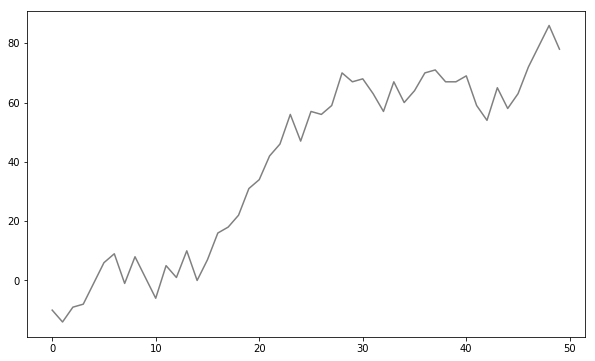
\includegraphics[width=.5\linewidth]{images/serie_exemplo.png}
    \source{Elaborado pelo autor}
\end{figure}

Considerando  então  que  a  série  apresentará  comportamento  estocástico,  é
possível  propor  modelos  que  serão  capazes  de  aproximar  o  comportamento
da  série.  Os  modelos  comumente  utilizados para  essa  tarefa  são  aqueles
probabilísticos, mais especificamente o ARIMA\@, proposto por \citeonline{box}.
Também é possível utilizar modelos criados a partir da aplicação de técnicas de
aprendizado de máquina,  que vem se apresentando como  uma alternativa poderosa
em muitas aplicações.

Com o  constante interesse na  aplicação e  a identificação das  capacidades de
técnicas de  aprendizado, fica  evidente a importância  de observar  como esses
modelos se comparam com os estatísticos. Dessa forma, o objetivo deste trabalho
foi comparar o desempenho de modelos  estatísticos e baseados em aprendizado de
máquina na previsão de uma  série de característica econômica. Especificamente,
foram  avaliados  o  modelo  estatístico  ARIMA  e  um  modelo  de  aprendizado
de  máquina baseado  em  redes  neurais artificiais  de  múltiplas camadas.  Os
resultados indicaram que  os modelos tiveram desempenhos  semelhantes nos dados
utilizados nesse trabalho.

% Como  forma de  comparar desempenhos  e  buscar compreender  as técnicas  que
% poderiam ser utilizadas para a previsão, este trabalho realizou a previsão de
% uma série de característica econômica utilizando ambas metodologias.

% TODO: Introduzir modelos ARIMA com exemplos de artigos

% FIXME Mais adequado na parte de trabalhos relacionados
%vez mais  notórias pelos bons resultados  que oferecem. \citeonline{artigoEx3}
%Em contrapartida, técnicas  de aprendizado de máquinas estão  se tornando cada
%aplicou  métodos  de aprendizado  de  máquina  possibilitando a  previsão  com
%bons  resultados. Pelo  fato  dos modelos  estatísticos fornecerem  resultados
%satisfatórios para predições e estarem bem difundidos na comunidade acadêmica,
%é  comum  que  trabalhos  como \citeonline{artigoEx4}  compare  os  resultados
%obtidos  a  partir  de  aprendizado   de  máquina  com  modelos  de  abordagem
%estatísticas. Para modelos de aprendizado se  destaca aqueles com uso de redes
%neurais  artificiais  por serem  capazes  de  obter bons  resultados  conforme
%analisado  por \citeonline{zhang},  o  autor ainda  apresenta outros  exemplos
%quais os autores obtiveram resultados superiores ao método estatístico.

O    restante   desta    monografia    está   organizada    como   segue.    No
\autoref{chap:fundTeor}  é apresentada  a  fundamentação  teórica do  trabalho,
incluindo os  principais métodos  de previsão  de séries  temporais empregados.
No  \autoref{chap:trab_relacionados} foram  apresentados  outros trabalhos  que
abordam  o   tema.  Já  no   \autoref{chap:desenv}  são  descritos   os  passos
metodológicos  empregados para  a desenvolvimento  tanto do  modelo estatístico
quanto  de  aprendizado  de  máquina.   Os  resultados  obtidos  com  base  nos
modelos construídos são apresentados  no \autoref{chap:result} e apresentada as
constatações  feitas  em ambos  modelos.  Por  fim, no  \autoref{chap:concl}  é
apresentada a conclusão do que foi realizado.

\chapter{Fundamentação teórica}\label{chap:fundTeor}

\section{Previsão}
Segundo  \citeonline{wiley},  o  processo  de previsão  pode  ser  dividido  em
diversas atividades, dispostas a seguir:

\begin{enumerate}
    \item Definição do problema\\
        Envolve  definir e  entender  a  tarefa de  previsão  a ser  realizada,
        considerando o prazo a ser previsto e definindo os dados necessários.
    \item Coleta dos dados\\
        Envolve a coleta  dos dados necessários de acordo com  as definições da
        atividade anterior.
    \item Análise dos dados\\
        Atividade de alta  importância para a seleção do  modelo mais adequado.
        Nessa  etapa   são  utilizadas  observações  gráficas   e  extração  de
        características para identificar padrões  que corroborem na escolha dos
        parâmetros. Também são identificadas  observações problemáticas e, caso
        necessário, aplicadas as devidas correções.
    \item Seleção e verificação do modelo\\
        A partir  da análise  feita na atividade  anterior, será  selecionado o
        modelo, analisando-se  também o comportamento com  os dados fornecidos.
        Como  método de  verificação são  utilizadas métricas  que favoreçam  a
        comparação.
    \item Avaliação do modelo\\
        Atividade na qual se avalia como  o modelo se comporta com novos dados,
        normalmente realizada  com observações  excluídas dos  dados utilizados
        nas atividades anteriores. As  observações separadas para avaliação são
        utilizadas apenas para essa finalidade.
    \item Publicação do modelo\\
        Com o modelo devidamente selecionado e avaliado, o mesmo é instalado em
        ambiente de produção, observando-se  as alterações necessárias para que
        novos dados sejam inseridos corretamente.
    \item Monitoramento do desempenho do modelo\\
        Deve-se continuamente  avaliar como  o modelo  aplicado se  comporta em
        relação ao ambiente, já que o ambiente é algo volátil.
\end{enumerate}

Essas  atividades  normalmente  são  realizadas em  ordem  como  exposta.  Vale
observar  ainda  que   se  os  resultados  da  atividade   de  avaliação  forem
insatisfatórios, deve-se  retornar à atividade  anterior e refazer  a avaliação
até que um modelo que obedeça às especificações seja encontrado.

\section{Séries temporais}\label{sec:seriesTemporais}

Como  exposto anteriormente,  séries  temporais são  compostas por  observações
sucessivas  feitas ao  longo do  tempo. Cabe  destacar ainda  que essas  séries
se  caracterizam   pelo  fato  de   suas  observações  serem   dependentes  das
observações  anteriores. Além  disso,  tais  séries demonstram  características
como  tendência e  sazonalidade.  A tendência  caracteriza  o comportamento  de
crescimento/decrescimento da série, o que  pode levar a observações futuras com
valores  menores ou  maiores. A  sazonalidade caracteriza  padrões cíclicos  em
função do tempo, comumente tomando períodos semanais, mensais ou anuais.

Uma série é descrita matematicamente pelo conjunto $\{X(t): t \in T\}$, podendo
$t$ ser  um tempo  contínuo ou  discreto. O  tempo $t$  é dito  contínuo quando
se  possui  observações  $X(t)$  para  todo $t$  em  $T$,  sendo  $T  \subseteq
\mathbb{R}^{+}$. O tempo $t$ é discreto  quando entre as observações $X(t_i)$ e
$X(t_{i+1})$ existe um  intervalo igual de tempo, normalmente dado  na forma de
uma sequência, $T = \{1, 2, \ldots, n\}$, sendo $n$ o número de observações.

Segundo  \citeonline{ehlers}, uma  série  temporal  classicamente é  decomposta
seguindo a \autoref{eq:timeseries}, sendo $t$ usado para denotar o tempo, logo,
é parte fundamental entender o comportamento segundo essas três componentes.

\begin{equation}
    \label{eq:timeseries}
    X_t = Tendência_t + Sazonal_t + Aleatório_t
\end{equation}

\subsection{Série estacionária}\label{sec:estacionaria}

Um  conceito   importante  para  a  análise   de  séries  temporais  é   o  seu
caráter  estacionário.  Um  processo  é  dito estacionário  se  todas  as  suas
características  comportamentais não  se  alteram ao  longo  do tempo.  Segundo
\citeonline{timeseriesExample} não existe  um limiar que defina  uma série como
estacionária, mas pode  definir como estacionário um processo  se desenvolve no
tempo em  torno da média, de  modo que a escolha  de uma origem dos  tempos não
é  importante.  Segundo  \citeonline{ehlers},  uma série  é  dita  estritamente
estacionária  quando  a  distribuição  de probabilidade  conjunta  de  $X(t_1),
\ldots, X(t_k)$ é igual a de $X(t_1 + \tau), \ldots, X(t_k + \tau)$.

Ainda segundo \citeonline{ehlers}, a definição  estrita de série estacionária é
dificilmente  aplicada,  então  usualmente  se utiliza  a  definição  de  série
fracamente estacionária,  que se define com  base no critério da  mesma possuir
função média constante. Dessa forma,  neste trabalho, foi utilizada a definição
de série fracamente estacionária para se tomar uma série como estacionária.

Em  termos matemáticos,  usa-se a  \autoref{eq:westacionaria} para  definir que
variância  de um  elemento da  série ($z_t$)  deve ser  semelhante à  média. Em
outras  palavras, o  deslocamento da  origem do  tempo $t$  por uma  quantidade
$\tau$ não  exerce efeito  na distribuição  conjunta da  série. Assim,  o valor
esperado para a série em determinado momento não será dada em função do tempo.

\begin{equation}
    \label{eq:westacionaria}
    E(z_t) = \mu_t = \mu
\end{equation}

% FIXME Dada em função de que??


%TODO Adicionar referência ao Livro Time Series by exmples

%TODO Adicionar referência ao teste de Dockey Fuller

% VALERIA: Deixe para mostrar o exemplo da série estacionária pós-diferenciação
% na seção que fala  sobre a diferenciação. Neste ponto do  texto ficou fora de
% contexto. Ou, se  vc quer mostrar um exemplo, mostre  uma série originalmente
% estacionária. Além  disso, nesse caso, vc  tem que explicar melhor  a figura.
% Por exemplo,  qual(is) característica(s) do  gráfico da série me  diz(em) que
% ela é  estacionária? Dizer  que a  observação do gráfico  é suficiente  não é
% suficiente. ;)

Segundo  \citeonline{timeseriesExample} embora existam testes  como o  de Dikey
Fuller  descrito  em  \citeonline{dickey}  para a  prova  de  estacionariedade,
é  suficiente  a observação  gráfica  da  série.  Caso  não seja  conclusiva  a
observação \citeonline{timeseriesExample} orienta obter  o gráfico da função de
autocorrelação,  e  se  observada  a  existência  de  mais  de  20  correlações
significativas pode-se classificar a série como não estacionária.

\subsection{Sazonalidade e tendência}

Conforme   definido  por   \citeonline{ehlers},   a  sazonalidade   caracteriza
repetições  de comportamento  de uma  série em  um período  $s$. A  presença da
sazonalidade,  em geral,  é facilmente  observada na  representação gráfica  da
série, conforme exemplificado no gráfico  da \autoref{fig:co2}. Nesse gráfico é
apresentada uma série  temporal real que registra a mudança  na concentração de
$CO_2$ na atmosfera. Observando o gráfico, é possível notar que há sazonalidade
de periodicidade anual, devido ao gráfico apresentar formato de serra e este se
apresentar em repetição anual.

Ainda  no  gráfico  da  \autoref{fig:co2},  também  é  possível  notar  que  há
uma  tendência de  crescimento na  série. Segundo  \citeonline{ehlers}, não  há
uma  definição exata  de  tendência, mas, normalmente, a  mesma é associada  ao
comportamento  de  mudança  das  observações  ao longo  de  um  vasto  período.
Uma  série  com tendência  pode  ser  descrita  como  a função  apresentada  na
\autoref{eq:tendencia},  na  qual $\alpha$  e  $\beta$  são os  coeficientes  e
$\epsilon_t$ é um erro aleatório  de distribuição normal. O coeficiente $\beta$
define a taxa de  crescimento da série, podendo ser dado  como um função global
ou definido localmente.

\begin{equation}
    \label{eq:tendencia} X_t = \alpha + \beta{}t + \epsilon_t
\end{equation}

% Um exemplo real de uma série  temporal que apresenta tendência e sazonalidade
% é mostrado  no gráfico  na \autoref{fig:co2}. Essa  série registra  a mudança
% na  concentração  de $CO_2$  na  atmosfera,  sendo,  portanto, uma  série  de
% característica natural.  Observando o gráfico,  é fácil notar a  tendência de
% crescimento da série e sua sazonalidade de periodicidade anual.

\begin{figure}[ht]
    \centering
    \caption{Leituras de $CO_2$ na atmosfera.}\label{fig:co2}
    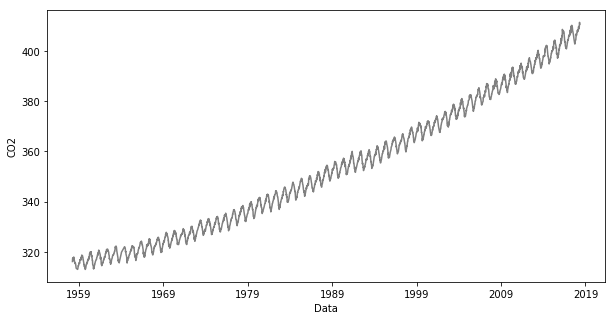
\includegraphics[width=.5\linewidth]{images/co2.png}
    \source{\citeonline{co2data}}
\end{figure}

\subsubsection{Filtros}

Em  algumas séries, a  tendência pode  não estar  evidente  devido ao  processo
aleatório. Por conta disso, pode ser  necessária a aplicação de filtros que têm
como objetivo obter  uma série suavizada que possibilite  observar a tendência.
Um desses filtros é apresentado na \autoref{eq:filtro}~\cite{ehlers}.

\begin{equation}
    \label{eq:filtro}
    y_t = \sum_{j = -q}^{s}{a_{j}x_{t+j}}
\end{equation}

Na \autoref{eq:filtro}, $a_j$  é um coeficiente a ser aplicado  a cada termo da
soma de forma a aplicar um peso a este, sendo observado que $\sum{a_j} = 1$.

A  \autoref{eq:yjfiltro}  é  conhecida  por   fornecer  o  cálculo  das  médias
móveis,  permitindo  suavizar  a  série,  mantendo  a  tendência.  A  aplicação
do  filtro  de médias  móveis  nos  dados das  leituras  de  $CO_2$ resulta  na
\autoref{fig:co2filtrado}.  Esta evidencia  de forma  independente a  tendência
após  a  remoção  da  sazonalidade,  por meio  da  suavização  utilizando  como
parâmetro $q$ seu período cíclico.

\begin{equation}
    \label{eq:yjfiltro}
    y_t = \frac{1}{2q + 1}\sum_{j=-q}^{q}{x_{t+j}}
\end{equation}

\begin{figure}[ht]
    \centering
    \caption{Leituras de $CO_2$ filtrada utilizando médias móveis com $q$ igual
        a $52$, devido à sazonalidade ser anual, ou seja, $52$
        semanas.}\label{fig:co2filtrado}
    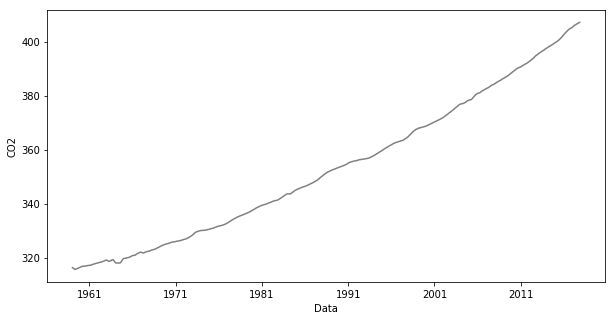
\includegraphics[width=.5\linewidth]{images/co2_filtered.png}
    \source{Elaborado pelo próprio autor a partir de \citeonline{co2data}}
\end{figure}

\subsubsection{Diferenciação}\label{sec:diff}

Outra tarefa a ser observada em relação  ao entendimento de tendência é a forma
na qual é removida. O método mais  simples para remoção da tendência é subtrair
de  cada valor  observado  o  valor do  seu  antecessor,  conforme descrito  na
\autoref{eq:diferenciacao}. Normalmente,  uma única diferenciação  é suficiente
para remover  a tendência, porém em  séries com componente sazonal  podem vir a
ser necessárias mais de uma em um \textit{lag} diferente.

\begin{equation}
    \label{eq:diferenciacao}
    y_t = x_t - x_{t-1}
\end{equation}

O gráfico  da \autoref{fig:co2diff} mostra o  resultado obtido para a  série de
leituras de $CO_2$ após uma diferenciação. Pelo gráfico é possível perceber que
a série resultante  se aproxima de uma série com  função média constante, dando
evidência a componente sazonal já que  a variação do gráfico apresenta um forte
comportamento repetitivo.

\begin{figure}[ht]
    \centering
    \caption{Série da leitura do $CO_2$ na atmosfera com uma
        diferenciação}\label{fig:co2diff}
    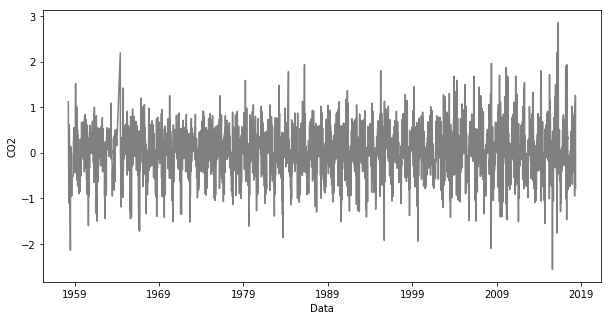
\includegraphics[width=.5\linewidth]{images/co2_diff.png}
    \source{Elaborado pelo autor a partir de \citeonline{co2data}}
\end{figure}

\section{Modelos probabilísticos}

Conforme  apresentado anteriormente,  as séries  temporais podem  ser previstas
utilizando-se modelos  estatísticos. Segundo \citeonline{ehlers}, isso  se deve
ao  seu caráter  estocástico, uma  vez  que cada  observação possui  correlação
com  as  observações  imediatamente   antecessoras,  diferentemente  de  séries
determinísticas, as quais têm seu estado  definido por uma função matemática ou
um sistema para o qual a saída é dependente apenas das entradas atuais.

Um modelo comumente utilizado para a  previsão de séries temporais é o ARIMA\@.
Descrito por  \citeonline{box}, esse  modelo caracteriza a  série em  termos de
três  parâmetros $(p,d,q)$,  sendo  cada  um associado  a  um  processo: $p$  é
associado a processos  autorregressivos, $d$ a integração e $q$  a processos de
médias móveis, embora de mesmo nome  este não tem qualquer associação ao filtro
de medias moveis.

A   definição  dos   valores   desses  parâmetros   depende   da  análise   das
características da  série. \citeonline{box}  descreveu algumas  ferramentas que
podem auxiliar nessa análise, entre elas a análise da função de autocorrelação.

\subsection{Função de autocorrelação}\label{sec:corre}

Como  o nome  sugere, a  função de  autocorrelação mede  a correlação  entre as
observações  de uma  série em  diferentes períodos.  Considerando-se uma  série
temporal $X$, calcula-se  a correlação entre seus valores com  uma defasagem de
tempo $k$,  sendo essa defasagem  a distância entre  o valor analisado  $X_t$ a
observação  $X_{t-k}$.  Por exemplo,  supondo  uma  série de  100  observações,
pode-se chamar de $X'$ a série  correspondente às 99 primeiras observações e de
$X''$ a série correspondente às últimas  99 observações. Nesse caso, tem-se uma
defasagem (ou \textit{lag}) de 1 período. Assim a função de autocorrelação será
dada segundo a \autoref{eq:autocorrelacao}.

\begin{equation}
    \label{eq:autocorrelacao}
    r_k = \frac{\sum_{t=1}^{n-k}{(x_t - \overline{x})(x_{t+k} -
    \overline{x})}}{\sum_{t=1}^{n}{(x_t - \overline{x})^2}}
\end{equation}

Segundo  \citeonline{ehlers},  a  função   de  autocorrelação,  quando  plotada
para  os  $k$-ésimos  primeiros  coeficientes,  é  chamada  de  correlograma  e
constitui-se em uma ferramenta importante para  as análises. Como um exemplo, a
\autoref{fig:correlogramaCo2}  apresenta o  correlograma  com  as 25  primeiras
defasagens das leituras de concentração  de $CO_2$ na atmosfera. Nesse gráfico,
também é exibido o intervalo de confiança de 95\% calculado para o correlograma
(destacado  em  azul).  Segundo   \citeonline{ehlers},  é  preciso  definir  um
intervalo de  confiança para o  correlograma para se definir  quais correlações
são relevantes e  quais não. De forma que todas  as correlações relevante estão
fora desse  intervalo de  confiança. Assim, se  todas as  correlações estiverem
dentro do  limite a série  é caracterizada como um  ruído branco, ou  seja, seu
comportamento não permite  modelagem. Para encontrar o  intervalo de confiança,
\citeonline{ehlers}  recomenda utilizar  a seguinte  equação $\pm{}2/\sqrt{n}$,
sendo $n$ o número de observações da série.

\begin{figure}[ht]
    \centering
    \caption{Gráfico da função de autocorrelação das leituras de
        $CO_2$}\label{fig:correlogramaCo2}
    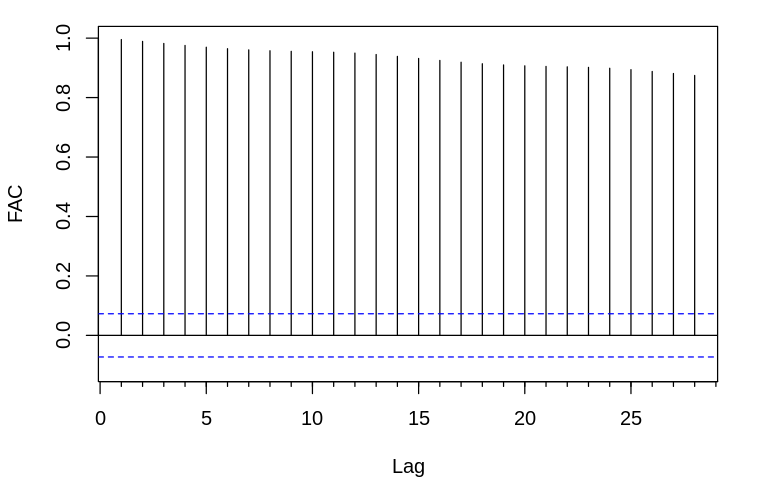
\includegraphics[width=.5\linewidth]{images/acf_co2.png}
    \source{Elaborado pelo autor a partir de \citeonline{co2data}}
\end{figure}

Para exemplificar como podemos utilizar a função de autocorrelação na definição
do modelo  podemos ver na  \autoref{fig:acfco2diff} a função  de autocorrelação
para a  primeira diferenciação da série  de leituras de $CO_2$.  Se observa que
após diferenciada, e removida a tendência, conseguimos observar o comportamento
sazonal, já  que a função  de autocorrelação apresenta correlações  positivas e
negativas em  uma distância que  pode ser entendida  como o período  cíclico da
série.

\begin{figure}[ht]
    \centering
    \caption{Gráfico de função de autocorrelação da diferenciação da série de
        $CO_2$}\label{fig:acfco2diff}
    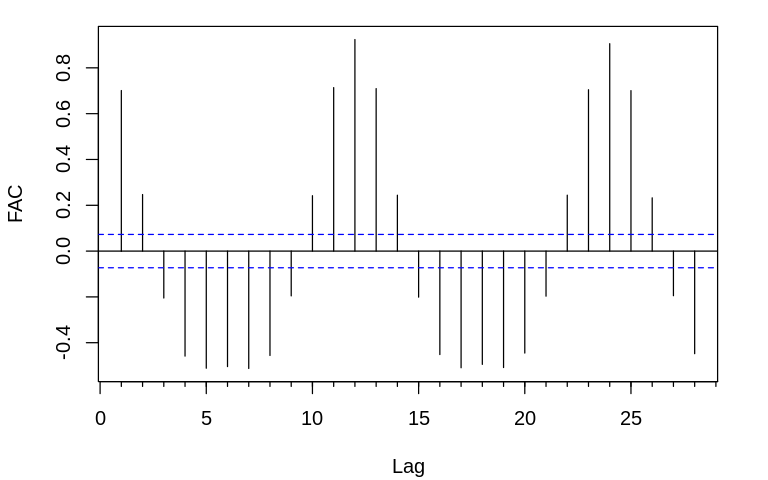
\includegraphics[width=.5\linewidth]{images/acf_co2_diff.png}
    \source{Elaborado pelo autor a partir de \citeonline{co2data}}
\end{figure}

\subsubsection{Função de autocorrelação parcial}

Durante  a análise,  outra função  relevante  é a  autocorrelação parcial.  Sua
definição segundo \citeonline{cryer} é dado  em \autoref{eq:facp}, onde $r_k$ é
a autocorrelação  da série $X$  no \textit{lag} $k$  e $\phi_{k,j}$ é  dado por
$\phi_{k-1, j}-\phi_{kk}\phi_{k-1,k-j}$.

\begin{equation}
    \label{eq:facp}
    \phi_{kk} = \frac{r_k-\sum_{j=1}^{k-1}{\phi_{k-1,j}r_{k-j}}}{1-\sum_{j=1}^{k-1}{\phi_{k-1,j}r_{j}}}
\end{equation}

\subsection{ARIMA}

O  modelo  ARIMA  já  introduzido  na seção  anterior  possui  três  parâmetros
essenciais $(p,q,d)$. Segundo \citeonline{rob} o modelo se diferencia de outros
por ser baseado na definições das autocorrelações da série.

\subsubsection{AR --- Processo auto regressivo}

Segundo  \citeonline{ehlers},  um  processo  $X_t$ é  chamado  auto  regressivo
de   ordem   $p$,   ou   $AR(p)$,   quando   temos   $X_t$   dado   segundo   a
\autoref{eq:aregressivo}.  Nesse caso,  $\alpha$  são os  coeficientes a  serem
calculados. O termo $\epsilon_t$ define  a componente aleatória, sendo definido
como ruido branco.

\begin{equation}
    \label{eq:aregressivo}
    X_t = \sum_{i = 1}^{p}{\alpha_{i}X_{t-i}} + \epsilon_t
\end{equation}

\subsubsection{MA --- Processo de médias móveis}

Segundo \citeonline{rob} é de forma  semelhante ao processo autorregressivo uma
regressão linear, com  coeficiente $\theta$, no entanto, esta  é aplicada sobre
os erros de  previsão $\epsilon_t$. Sendo associada ao filtro  de médias móveis
por conta de ser descrito também como um filtro dos os erros de previsão.

\begin{equation}
    \label{eq:pmediasmoveis}
    X_t = \epsilon_t - \theta_1\epsilon_{t-1} - \theta_2\epsilon_{t-2} - \cdots - \theta_{q}\epsilon_{t-q}
\end{equation}

\subsubsection{ARMA --- Modelo misto}

Combinando os processos AR e MA, podemos obter um modelo extremamente útil para
descrever  séries temporais.  E a  junção dos  modelos pode  ser expressa  pela
\autoref{eq:arma}.

Então, segundo \citeonline{timeseriesExample}, se  considerarmos $X_t$ como uma
série estacionária, teremos  o processo AR relacionando a  observação atual com
as  $p$ observações  anteriores; e  o  processo MA  apresentando as  defasagens
passadas.

\begin{equation}
    \label{eq:arma}
    X_t = \sum_{i = 1}^{p}{\alpha X_{t-i}} + \epsilon_t - \sum_{j = 1}^{p}{\theta \epsilon_{t-i}}
\end{equation}

\subsubsection{Integração}

Em  casos  que a  série  analisada  apresenta  não estacionariedade, segundo  a
definição dada  na \autoref{sec:estacionaria}, é necessária  a transformação em
uma série estacionária. Isso pode  ser facilmente realizado utilizando o método
de  diferenciação  descrito na  \autoref{sec:diff}.

Segundo \citeonline{rob} podemos definir  a diferenciação utilizando o operador
de \textit{backshift}, $B$, definido na \autoref{eq:backshift}. Assim definimos
a \autoref{eq:diffback}  como a  primeira diferenciação  da série  utilizando o
operado $B$.

\begin{equation}
    \label{eq:backshift}
    By_t = y_{t-1}
\end{equation}

\begin{equation}
    \label{eq:diffback}
    y'_t = y_t - y_{t-1} = y_t - By_t = (1-B)y_t
\end{equation}

Diferenciações de maior ordem são definidas por $(1-B)^dy_t$.

Combinando  os  processos apresentados  podemos  descrever  o ARIMA  segundo  a
\autoref{eq:ARIMA}.

\begin{equation}
    \label{eq:ARIMA}
    (1 - \alpha_1B-\cdots-\alpha_pB^p)(1-B)^dy_t=(1+\theta_1B+\cdots+\theta_qB^q)\epsilon_t
\end{equation}

\subsection{Seleção do modelo}

De acordo  com \citeonline{box},  a identificação  do modelo  pode ser  feita a
partir da  análise gráfica  da função  de autocorrelação, FAC,  e da  função de
autocorrelação parcial,  FACP, que  foram apresentados  na \autoref{sec:corre}.
Podendo,  ainda,  contar  com  a  ajuda de  outros  testes  para  validação  da
estacionariedade da série.

O método proposto por \citeonline{box} observa o comportamento das correlações.
Desta forma para identificar  a ordem do AR é suficiente  analisar se o gráfico
do FAC apresenta decaimento exponencial e FACP apresenta uma quebra a partir do
$p$-ésimo valor do  gráfico. Já a identificação da ordem  do processo de médias
móveis  é feita  de modo  semelhante,  porem o  $q$  é dado  pela elemento  que
apresenta  a quebra  no gráfico  do FAC  enquanto o  gráfico do  FACP apresenta
decaimento exponencial.

Se não for  possível identificar a série a partir  deste procedimento, pode ser
que a  série apresente  tendência. No  caso de  existir tendência  é necessária
a  realização  de  uma  ou  mais diferenciações,  com  essa  nova  série  agora
estacionaria é refeito as verificações e determinadas as ordens.

% FIXME Tem que achar uma referencia coerente para definição do modelo

Para os casos descritos  o modelo obtido é da forma  $AR(p)$ ou $MA(q)$, porem,
em casos  de modelos híbridos  ambas funções devem apresentar  comportamento de
quebra  a  partir  do  $q$-ésimo  para  o  FAC  e  $p$-ésimo  para  FACP\@.  Na
\autoref{tab:facpacf} temos  esse procedimento  de seleção  do modelo  de forma
sumarizada.

\begin{table}[ht]
    \centering
    \caption{Modelo conforme FAC e FACP}\label{tab:facpacf}
    \begin{tabular}{l l l}
        \multicolumn{1}{c}{Modelo} & \multicolumn{1}{c}{FAC} & \multicolumn{1}{c}{FACP} \\
        \toprule
        Série aleatória  & 0                           & 0                        \\
        AR (p)           & decaimento exponencial      & 0 após $p$ \textit{lags} \\
        MA (q)           & 0 após $q$ \textit{lags}    & decaimento exponencial   \\
    \end{tabular}
    \source{\citeonline{ehlers}}
\end{table}

Porem, segundo  \citeonline{vinay} essa  forma nos  fornece modelos  que servem
somente  como uma  boa aproximação.  Para determinação  de um  modelo realmente
eficiente  pode  ser necessário  a  execução  de  um  grande número  de  testes
exaustivos.  E, utilizando-se  de  alguma métrica  selecionar  aquele que  seja
parcimonioso  e  forneça  bons  resultados.  Segundo  \citeonline{rob}  deve-se
da  minimizar   o  critério  de   informação  de  Akaike  definido   segundo  a
\autoref{eq:aic}, sendo $L$ o \textit{likelihood} do modelo.

\begin{equation}
    \label{eq:aic}
    AIC = -2\log{L}+2(p+q+1)
\end{equation}

\subsection{Determinação dos coeficientes}

Por fim, para completa construção do modelo apresentado na \autoref{eq:arma}, é
necessária a obtenção dos coeficientes  do processo autorregressivo e de médias
móveis. Para essa  tarefa, segundo \citeonline{vinay}, é comum  a utilização do
estimador de \textit{likelihood}, ou mais  precisamente a maximização da função
de \textit{likelihood}.

Essa  maximização   é  descrita   por  \citeonline{statiticalML}   da  seguinte
forma:  considerando  uma função  $q(x;\theta)$, que  nos retorna  a  densidade
probabilística de uma entrada $x$ com um conjunto de parâmetros a ser otimizado
$\theta$ de dimensão $b$, o objetivo é a maximização da \autoref{eq:likelihood}
que nos retorna a capacidade dos parâmetros em aproximar a série.

\begin{equation}\label{eq:likelihood}
    L(\theta) = \prod_{i=1}^{n}{q(x_i;\theta)}
\end{equation}

\subsubsection{Equação de Yule Walker}

Outra forma de  obter os coeficientes do processo autoregressivo  é através das
equações  de Yule  Walker. \citeonline{eshel}  descreve como  é realizado  esse
procedimento. De forma geral os coeficientes podem ser encontrados utilizando a
\autoref{eq:yulewalker}, sendo $r_k$ as autocorrelações obtidas na FAC da série
e $\alpha$  os coeficientes do  AR\@. Esta  forma de encontrar  os coeficientes
torna evidente a relação entre a análise das correlações e o modelo.

\begin{equation}
    \label{eq:yulewalker}
    \begin{pmatrix}
        r_1\\
        r_2\\
        \vdots\\
        r_{p-1}\\
        r_p
    \end{pmatrix} =
    \begin{pmatrix}
        1 & r_1 & r_3 & \cdots & r_{p-2} & r_{p-1} \\
        r_1 & 1 & r_1 & \cdots & r_{p-3} & r_{p-2} \\
        & & \vdots & & \vdots & \\
        r_{p-2} & r_{p-3} & r_{p-4} & \cdots & 1 & r_1 \\
        r_{p-1} & r_{p-2} & r_{p-3} & \cdots & r_1 & 1 \\
    \end{pmatrix}
    \begin{pmatrix}
        \alpha_1\\
        \alpha_2\\
        \vdots\\
        \alpha_{p-1}\\
        \alpha_p
    \end{pmatrix}
\end{equation}

\section{Aprendizado de Máquina}

Computadores se utilizam de algoritimos  para realizar processamento de dados e
solucionar  problemas.  Porém,  para  determinados problemas,  não  é  possível
definir um  algoritmo, seja porque o  seres humanos não conseguem  explicar seu
conhecimento, ou esse conhecimento é  muito complexo para ser  explicitado, ou,
ainda, porque  o conhecimento  e a  solução do  problema muda  com o  passar do
tempo.  Um exemplo  de tal  situação seria  a classificação  de um  e-mail como
\textit{spam} ou legitimo.  Definir as características que fazem  um e-mail ser
considerado \textit{spam}  pode se  tornar um problema complexo, especialmente,
considerando-se que  a definição  de \textit{spam}  pode variar  com o  tempo e
com o usuário.

Conforme \citeonline{ethem}, tarefas como a identificação de \textit{spam}, que
não apresentam  uma solução  evidente, mas  que podem  ser resolvidas  por meio
da  identificação  de padrões  a  partir  de um  conjunto  de  dados, são  boas
candidatas à aplicação de técnicas  de aprendizado de máquina. Entretanto, para
classificarmos esse sistema como inteligente, não é suficiente que o mesmo seja
capaz de inferir padrões de uma base, precisamos que este, ainda, seja capaz de
se adaptar a mudanças e aprender com isso.

Como forma  de apresentar  os usos  e entender o  funcionamento de  técnicas de
aprendizado \citeonline{ethem} coloca os seguintes exemplos de aplicação.
\begin{itemize}
    \item Classificação\\
        Em aplicações  financeiras a  análise de risco  é parte  fundamental da
        manutenção  de  uma boa  lucratividade.  Podemos  utilizar técnicas  de
        aprendizado  de  máquina  para  reconhecer um  padrão  em  um  conjunto
        pré  existente  já  classificados  de aplicações  problemáticas  e  não
        problemáticas, e  generalizar a  partir deste conjunto  para aplicações
        ainda não observadas.
    \item Regressão\\
        A previsão de custo de um  carro usado, pode exemplificar como técnicas
        de aprendizado  de máquina são  capazes de partindo  de características
        desses automóveis,  fornecer uma  boa estimativa  do custo  do veiculo.
        No  caso  essa  estimativa  é um  valor  continuo,  diferentemente  das
        tarefas  de  classificação  onde  o objetivo  é  encontrar  uma  classe
        discreta que  defina a entrada.  De forma semelhante à  classificação é
        utilizado um conjunto pré existentes para poder ensinar ao algorítimo o
        comportamento da saída com relação a entrada.
    \item Aprendizado não supervisionado\\
        Enquanto os  exemplos anteriores  envolviam um  conjunto de  dados para
        identificação  do  padrão  do  mapeamento da  entrada  para  uma  saída
        ,  no  aprendizado  não  supervisionado  o  objetivo  é  reconhecer  na
        entrada  um  padrão  ainda  desconhecido. No  exemplo  apresentado  por
        \citeonline{ethem} é  realizado o agrupamento  de clientes com  base em
        seus  comportamentos, assim  identificando  clientes com  comportamento
        semelhante e  permitindo criar  estrategias de  venda pontuais  a estes
        grupos.
    \item Aprendizado por reforço\\
        Aplicado em casos onde uma única ação não é suficiente para definir uma
        solução, como  em jogos  eletrônicos. Definindo  então uma  politica de
        boas  ações, por  exemplo, um  robô encontrando  um caminho,  este deve
        fazer varias tentativas até encontrar  um caminho que seja satisfatório
        e aprender como identificar a sequencia de ações que levam a ele.
\end{itemize}

Um    exemplo   real    de    uso    de   aprendizado    de    máquina   é    a
identificação  de   caracteres  numéricos  escritos  à   mão.  Apresentado  por
\citeonline{machineLearning},  esse  exemplo é  descrito  como  um problema  de
classificação no qual uma imagem de dimensões $28 \times 28$ pixeis é dada como
entrada para  um sistema que  deve atribuir uma  categoria que descreve  qual o
número que  a figura representa. Um  conjunto de exemplos de  tais imagens pode
ser visto  na \autoref{fig:numeroClassi}. No  caso o algoritimo a  ser aplicado
tem base  em aprendizado supervisionada, já  que este dispõe de  um conjunto já
classificado.

\begin{figure}[ht]
    \centering
    \caption{Exemplo de entrada para o algorítimo de
        classificação}\label{fig:numeroClassi}
    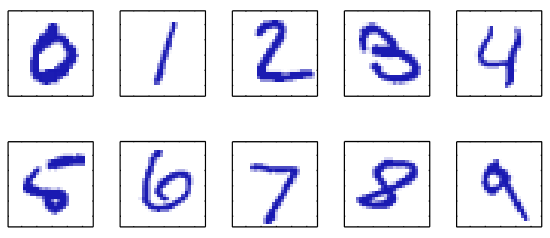
\includegraphics[width=.5\linewidth]{images/numeroClassificacao.png}
    \source{\citeonline{machineLearning}}
\end{figure}

No exemplo apresentado na \autoref{fig:numeroClassi}, podemos entender a tarefa
como  um sistema  no qual  $x$ é  a entrada  e $\hat{Y}$  é conjunto  de saída.
Matematicamente,  podemos expressar  da forma  vista na  \autoref{eq:sisCla}. A
saída será na forma  de um conjunto de números variando de 0  a 1 expressando a
probabilidade  de  $x$ pertencer  à  classe  $\hat{Y}_i$  onde  $i$ é  o  valor
expressado na imagem.

\begin{equation}
    \label{eq:sisCla}
    f(x) = \hat{Y}
\end{equation}

Prever o próximo valor de uma  série pode ser realizado considerando o conjunto
de entrada  como os valores  anteriores e o de  saída os valores  previstos. Se
assemelhando  a  tarefa  de  regressão.  Como  exemplo  se  dermos  um  sistema
$f{(x_{t-1})}  = x_t$  e tendo  um conjunto  de $n$  observações anteriores,  é
possível obter um modelo com base na identificação de padrões encontrados nesse
conjunto.

Na  proxíma subseção  é  detalhado  o algoritimos  de  aprendizado de  máquina,
baseado em redes  neurais aritificais com foco mais especifico  em problemas de
regressão. Abordadndo também as técnicas de aprendizado utilizdas.

\subsection{Redes Neurais artificiais}

Segundo  \citeonline{haykin2009}, a pesquisa  em  redes  neurais artificiais  é
motivada pelo entendimento que o cérebro  humano realiza o processamento de uma
forma  completamente diferente  dos computadores  convencionais. Essa  forma de
realizar  o processamento  realizado  pelo cérebro  é  altamente complexa,  não
linear e altamente paralela. A unidade de processamento e organização básica de
um cérebro são  os neurônios. O autor ainda lhe  confere superior capacidade na
realização de  tarefas como  reconhecimento de padrões  do que  os computadores
digitais.

Os animais  já nascem com  o cérebro possuindo  certa estruturas que  estes vão
precisar  durante sua  vida.  Porém este  é concebido  ainda  de maneira  muito
plástica, ou seja, possuindo ainda a capacidade de, na fase de aprendizado, ser
capaz de se adaptar ao contexto em  que vai se desenvolver. Este mesmo conceito
de  plasticidade  também  foi  utilizado  para a  modelagem  de  redes  neurais
artificiais~\cite{haykin2009}.

\subsubsection{\textit{Perceptron}}

Como  já  colocado, as  redes  neurais  possuem  o  neurônio como  elemento  de
processamento. Isto,  em redes artificiais, associamos  ao \textit{perceptron}.
Descrito  primeiramente por  Rosenblatt em  1962,  tem sua  função definida  em
\autoref{eq:perceptron},  sendo  dado  como  a soma  ponderada  por  $w_i$  das
entradas, $x_i$.  Visualmente, o  \textit{perceptron} é representado  segundo a
\autoref{fig:perceptron}.

\begin{equation}\label{eq:perceptron}
    v(x) = \sum_{i=1}^{m}{w_i  x_i + b}
\end{equation}

\begin{figure}[ht]
    \centering
    \caption{Representação gráfica de um \textit{perceptron}}\label{fig:perceptron}
    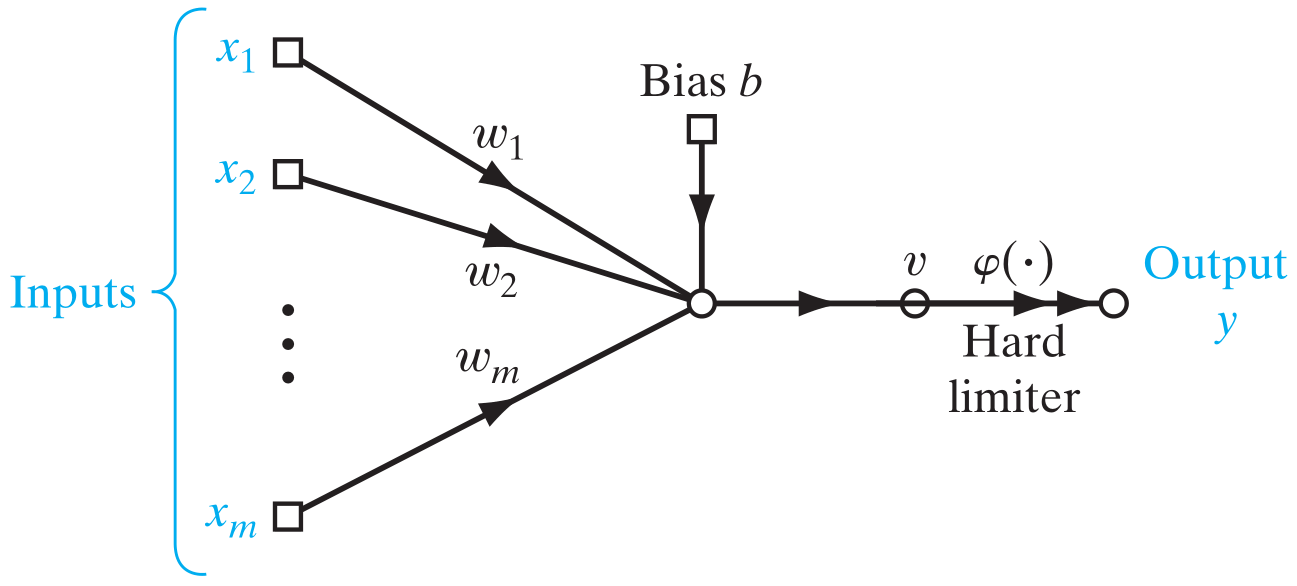
\includegraphics[width=.5\linewidth]{images/perceptron.png}
    \source{\citeonline{haykin2009}}
\end{figure}

Após a  soma ponderada,  é aplicada  ao resultado $v$  uma função  de ativação.
Classicamente, essa função é  dada como uma função degrau, ou  seja, se o valor
resultante da soma ponderada for maior que um valor determinado, o resultado do
processamento do neurônio artificial é 1, caso contrário, é 0~\cite{knight}.

Um exemplo dessa função degrau é dada da forma da \autoref{eq:funLimiar}. Nesse
exemplo, a função  resulta em 1, quando o valor  do \textit{perceptron} é maior
que 0; e 0, quando menor.

\begin{equation}
    \label{eq:funLimiar}
    o(v) = \left\{
        \begin{array}{lr}
            1 & :se\  v(x) > 0\\
            0 & :se\  v(x) < 0
        \end{array}
    \right.
\end{equation}

Outras  duas  funções de  ativação  importantes  são  a  logística e  a  linear
retificada,   respectivamente,   apresentadas   em   \autoref{eq:logistica}   e
\autoref{eq:relu}. As duas  apresentam a característica de  serem continuas, no
entanto, a  função logística se limita  ao intervalo de  0 e 1, enquanto  que a
linear retificada só é limitada inferiormente em 0.

\begin{equation}
    \label{eq:relu}
    o(v) = \left\{
        \begin{array}{lr}
            v & :se\  v(x) > 0\\
            0 & :se\  v(x) < 0
        \end{array}
    \right.
\end{equation}

\begin{equation}
    \label{eq:logistica}
    o(v) = \frac{1}{1+e^{-x}}
\end{equation}

Graficamente   podemos  representar   as   funções  de   ativação  conforme   a
\autoref{fig:ativacao}. 

A  função degrau  embora extremamente  simples só  tem eficacia  em tarefas  de
classificação, já que  regressões demandam dados contínuos e  esta possui saída
discretizada.

Se a aplicada  a função logística na saída é  necessário dimensionar o conjunto
de treinamento para o intervalo 0 e 1.

\begin{figure}[ht]
    \centering
    \caption{Funções de ativação}\label{fig:ativacao}
    \begin{subfigure}{.3\textwidth}
        \centering
        \caption{Função linear retificada}
        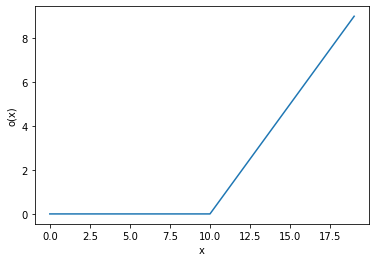
\includegraphics[width=.9\linewidth]{images/relu.png}
    \end{subfigure}
    \begin{subfigure}{.3\textwidth}
        \centering
        \caption{Função logística}
        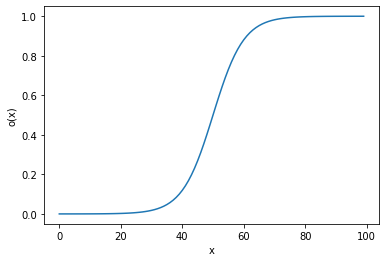
\includegraphics[width=.9\linewidth]{images/sigmoid.png}
    \end{subfigure}
    \begin{subfigure}{.3\textwidth}
        \centering
        \caption{Função degrau}
        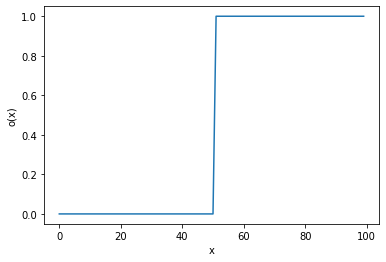
\includegraphics[width=.9\linewidth]{images/degrau.png}
    \end{subfigure}
    \source{Elaborado pelo autor}
\end{figure}

Ainda segundo  \citeonline{knight}, o \textit{perceptron} se  caracteriza pelos
pesos e pela definição  do valor da função de ativação,  enquanto o processo de
aprendizagem se caracteriza pela modificação desses pesos e valores.

Porém a  utilização de  sistemas simples com  somente um  \textit{perceptron} é
insuficiente  na  solução  de muitos  problemas.  Segundo  \citeonline{knight},
o  \textit{perceptron}  sozinho é  incapaz  de  traçar hiperplanos  capazes  de
resolver problemas  de classificação não  lineares. No exemplo  apresentado por
\citeonline{knight}, é demonstrado que, enquanto um neurônio artificial é capaz
de reproduzir corretamente o comportamento de um porta logica E ou OU, este não
consegue sintetizar uma  porta OU-exclusivo. Com isso, é definido  um limite ao
\textit{perceptron}.

\subsubsection{Redes neurais \textit{feedforward}}

Ainda considerando  a incapacidade do  \textit{perceptron} de uma  única camada
modelar  algumas classes  de  problemas, \citeonline{knight}  apresenta que  se
empregado  mais de  uma camada  seremos  capazes, então,  de representar  esses
problemas mais  complexos. A  essa arquitetura de  organização de  neurônios se
dá  o  nome  de  redes  neurais de  múltiplas  camadas.  Quando  a  alimentação
dela  é na  direção  da entrada  para  a saída  será  classificada também  como
\textit{feedforward}.

Podemos  entender  uma  rede  neural   de  múltiplas  camadas  em  três  partes
essenciais: a camada de entrada, a escondida  e, por último, a camada de saída.
A  camada de  entrada é  aquela que  recebe as  características do  conjunto de
dados. O nome de \textit{feedforward} é  dado devido à entrada ser apresentada,
primeiramente, a camada de  entrada e as ativações fluírem até  a saída. Logo o
resultado da  rede será encontrado  na camada de saída  após passar por  toda a
rede em  uma única  direção. Visualmente,  pode-se expressar  a rede  segundo a
\autoref{fig:neuralNetwork}.

\begin{figure}[ht]
    \centering
    \caption{Representação da ligação entre \textit{perceptron} em uma rede
    neural}\label{fig:neuralNetwork}
    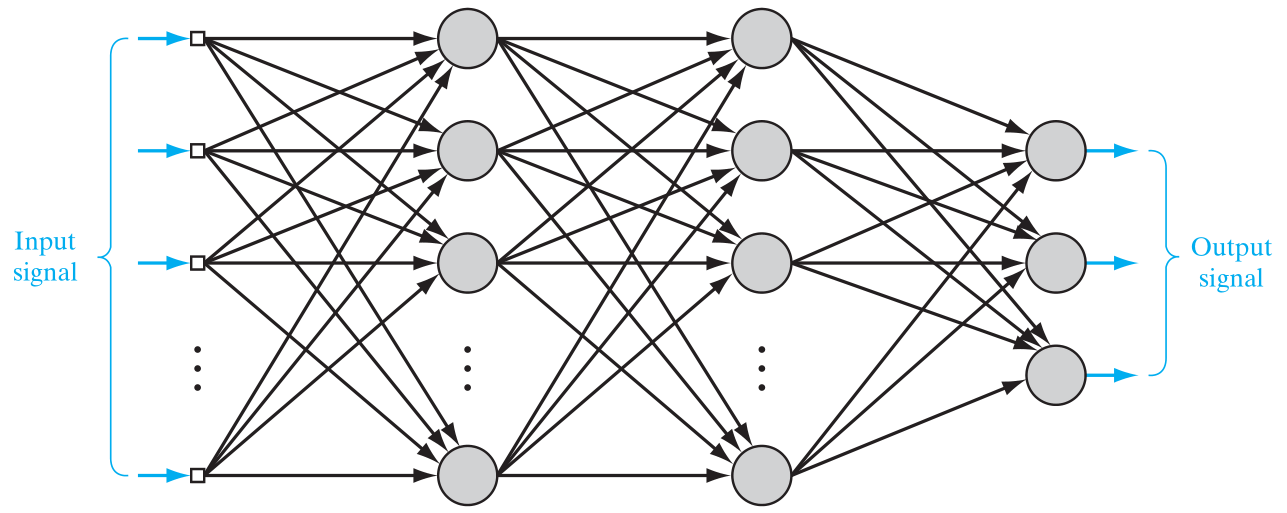
\includegraphics[width=.5\linewidth]{images/neuralNetwork.png}
    \source{\citeonline{haykin2009}}
\end{figure}

Sendo os  parâmetros a  serem definidos  em uma rede  neural somente  os pesos,
$w_i$. Define-se que  estes serão inicializados como  valores aleatórios, sendo
reajustados uma vez a cada passagem do aprendizado.

Para avaliação dos pesos, é necessário  utilizar uma função de cálculo do erro.
Como este trabalho consiste na realização  de regressão, o cálculo do erro será
dado pela função de erro quadrado  médio conforme \autoref{eq:mse}, sendo $Y$ o
conjunto de treinamento, $\hat{Y}$ o valor previsto e $n$ o tamanho do conjunto
de treinamento.

\begin{equation}\label{eq:mse}
    MSE = \frac{1}{n}\sum_{i=1}^{n}{{(Y_i - \hat{Y}_i)}^2}
\end{equation}

\subsubsection{Retro propagação}

A atualização  dos pesos ocorre  a cada iteração  sobre os valores  de entrada.
Assim,  suas  saídas  são  comparadas  com  os  valores  reais  e  computado  o
valor  do erro.  Tendo os  valores  dos erros,  $L$,  esse valor  é aplicado  a
\autoref{eq:backpropagation} e, então, os pesos  da rede neural são atualizados
para a  nova iteração,  sendo aplicado  uma taxa  de aprendizado,  $\alpha$, ao
valor que serão corrigidos os pesos.

\begin{equation}\label{eq:backpropagation}
    w_{n+1} = w_n - \alpha \frac{\partial L(x,w_t)}{\partial w_t}
\end{equation}

\subsubsection{Avaliação e seleção do modelo}

Após  o treinamento  do  modelo,  deve-se avaliar  a  capacidade  do modelo  de
generalização para dados ainda não apresentados a ele. Esse conceito é dado por
\citeonline{haykin2009} como sendo um dos  principais objetivos de um modelo de
redes neurais.

Para se avaliar a capacidade de generalização, é separada uma porção dos dados,
normalmente, em uma  proporção de 30\%. Assim, durante a  etapa de treinamento,
utiliza-se  a  porção maior  dos  dados  e, após  o  modelo  estar treinado,  é
verificado a qualidade  utilizando a função de erro,  já definida anteriormente
na \autoref{eq:mse}, mas agora no conjunto de teste (porção menor dos dados).

Já  que, durante  a  etapa  de  aprendizado, o  modelo  só  obterá  informações
do  conjunto  de   trinamento,  faz-se  necessário   algumas  estratégias  para
impedir  que  o  modelo  se  especialize no  conjunto.  Essa  especialização  é
conhecida por \textit{overfit}, o que pode  causar a incapacidade do  modelo em
prever  corretamente  os  dados  que  ainda não  lhe foram  apresentados.  Para
impedir  isto, podemos  realizar   os  seguintes  procedimentos  descritos  por
\citeonline{deepLearning}:

\begin{enumerate}
    \item Validação cruzada\\
        O conjunto de  dados é divido em $k$ subconjuntos,  \textit{folds}, e a
        rede neural é  treinada utilizando $k-1$ \textit{folds}.  O modelo será
        validado  no  subconjunto deixado  de  fora  do treinamento.  Ocorrerá,
        ainda,  a  mudança  do  conjunto que  servirá  para  validação.  Assim,
        impede-se  que a  rede se  especialize  em um  conjunto especifico.  Na
        \autoref{fig:crosvalidation}, o conjunto de  entrada é dividido em três
        \textit{folds} e o  treinamento é realizado nas  três divisões criadas,
        sendo os  conjuntos em  azul utilizados para  treinamento e  aqueles em
        vermelho  utilizados  para  avaliar  o modelo.  Essa  avaliação  ocorre
        conforme um  método, $L_{cv}$,  que reúne  a avaliação  de todos,  $L =
        L_{cv}(L_1, L_2, L_3)$.

        \begin{figure}[ht]
            \centering
            \caption{Divisão da entrada em três\textit{folds}}\label{fig:crosvalidation}
            \includegraphics[width=.5\linewidth]{images/cross_validation.png}
            \source{Elaborado pelo autor}
        \end{figure}

    \item Regularização\\
        Tem como objetivo manter os pesos do modelo minimizados. O procedimento
        consiste em  alterar a função do  erro adicionando a ela  os custos dos
        pesos,  isso é  feito conforme  a \autoref{eq:regL1}.  Em que  $L$ é  a
        função de perda  anterior e $L_{reg}$ a regularizada, $w$  são os pesos
        do modelo  e $\lambda$  é a  taxa de  regularização. Se  selecionado um
        valor muito  alto, os pesos  tenderão a $0$ e  o efeito prático  será o
        contrário ao desejado. Consequentemente, o modelo passará a ser incapaz
        de representar também o conjunto de entrada.

        \begin{equation}\label{eq:regL1}
            L_{reg} = L + \lambda \sum{|w|}
        \end{equation}
\end{enumerate}

Como já foi explicitado, existem diversas  definições a serem realizadas para a
produção do modelo.  Deve-se, então, realizar testes nesses  diversos modelos e
escolher aquele  que melhor se  adeque segundo a  função de erro  definida. Tal
procedimento é conhecido  por busca em grade, realizando a  avaliação do modelo
para todas as combinações de parâmetros definidos na grade.

\chapter{Trabalhos relacionados}\label{chap:trab_relacionados}

Com objetivo de  entender e analisar como os modelos  estudados se comportavam,
foram analisados  diversos trabalhos.  Sendo inicialmente avaliados  os estudos
com foco  na utilização  dos modelos  estatísticos; e, após  isso, a  busca por
textos que  observaram o  comportamento de modelos  de aprendizado  de máquina.
Além  desses casos,  foram buscados  trabalhos  que utilizam  ambos modelos  em
formato de comparação, semelhante ao objetivo deste trabalho.

% TODO: Finalizar esse trabalho relacionado

Em  \citeonline{giebel2011state}  o autor  realiza  a  predição da  geração  de
energia eólica, a produção é dada  em função da capacidade na região instalada,
o vento,  no entanto,  é um  elemento volátil e  sendo assim  existirá momentos
quais o  uso de  outras fontes  será necessária, contudo,  é preciso  ter certo
conhecimento prévio,  pois, o  ligamento de  uma usina  como aquelas  movidas a
gasóleo podem levar  até duas horas. Logo  prever duas horas a  frente pode ser
crucial para garantir o abastecimento de energia a uma região, podendo impactar
no cotidiano e economia de uma população.

\citeonline{vinay}  utilizou   modelos  ARIMA   e  suas  variações,   SARIMA  e
ARIMA-GARCH, para  previsão de tráfego em  rodovias. Um de seus  desafios foi a
necessidade de predição em tempo real, ou seja, o modelo tinha de ser obtido ao
mesmo tempo  que os dados eram  gerados. Ele identificou que  modelos ARIMA tem
uma alta complexidade para serem encontrados,  já que ele usou uma abordagem de
busca em  grade para  identificar o  modelo adequado,  utilizando a  métrica de
média das somas quadradas dos erros para avaliação.

\citeonline{reza}  propôs um  modelo  ARIMA modificado, acrescentando ao  valor
previsto a  soma das médias dos  erros para encontrar um  modelo mais adequado.
Sua  abordagem obteve  resultados  melhores que  aqueles observados  utilizando
somente ARIMA\@.

Já \citeonline{matias} comparou  ARIMA com outros modelos  de base estatística.
Além disso,  propôs um modelo híbrido  entre eles, para previsão  de demanda de
táxis na cidade  de Porto em Portugal, com objetivo  de melhorar a distribuição
dos táxis. Um de seus desafios  foi combinar a informação de geolocalização com
as séries das demandas por corridas. Como  resultado, ele foi capaz de obter um
erro inferior a 26\% na previsão de corridas utilizando o modelo proposto.

Quanto  à  utilização  de  redes   neurais,  podemos  observar  o  trabalho  de
\citeonline{zhangbco}. Nesse  trabalho, foi  observado o  desempenho do  uso de
redes neurais  utilizando o algoritimo de  retro propagação e outro  baseado em
algoritimos naturais. A série utilizada foi  a do índice S\&P500. Foi comparada
a previsão  entre um e  quinze dias adiante. O  modelo neural utilizado  foi de
três camadas, com 9  neurônios na camada de entrada, 3 na  camada escondida e 1
na de saída.  O modelo proposto utilizando o algoritimo  natural teve resultado
superior para todas as análises.

\chapter{Desenvolvimento}\label{chap:desenv}

Como  colocado  na \autoref{sec:seriesTemporais},  a  capacidade  de se  prever
séries temporais tem grande importância, e  uma de suas principais aplicações é
na  previsão de  indicadores  econômicos.  O S\&P500,  um  índice mantido  pela
Standard \&  Poor's desde 1923,  indexa os valores de  500 ativos em  bolsas de
valores e  serve como  um indicador  geral do  comportamento do  mercado. Logo,
foram  obtidos os  dados do  S\&P500 para  comparar os  modelos apresentados  e
observar o seu desempenho de previsão.

Durante  toda  a  etapa  de  desenvolvimento,  foi  utilizada  a  linguagem  de
programação   python\footnote{\url{https://www.python.org}}  em   conjunto  com
jupyter  para  a  análise  das   séries,  produção  dos  modelos  e  avaliação.
Especificamente,   para    os   modelos   probabilísticos    foram   utilizadas
as    biblioteca   statsmodels\footnote{\url{https://www.statsmodels.org}}    e
tensorflow\footnote{\url{https://www.tensorflow.org/}}   para  os   modelos  de
aprendizado de  máquina. Além delas,  foram utilizadas as  bibliotecas seaborn,
para produção dos gráficos, e pandas em conjunto com numpy e scikit-learn, para
importar e realizar as modificações necessárias dos dados.

Os           dados            da           série            podem           ser
obtidos      online\footnote{\url{https://datahub.io/core/s-and-p-500}}.     Na
\autoref{fig:sp500}, apresenta-se  as observações do índice  S\&P500 utilizadas
durante o desenvolvimento deste trabalho.

Para simplificar as tarefas realizadas no  decorrer deste trabalho, os dados da
série foram dimensionados no intervalo entre 0  e 1. Para isso, foi utilizado o
método \texttt{MinMaxScaler}  da biblioteca  sklearn, que  matematicamente pode
ser representado como visto na \autoref{eq:minmaxscaler}, sendo $MAX$ e $MIN$ o
intervalo  que definimos  para  a série  e  a função  $\min$  e $\max$  capazes
respectivamente de apresentar o menor e maior elemento do conjunto.

\begin{equation}
    \begin{split}\label{eq:minmaxscaler}
        &X_{std} = \frac{X - \min X}{\max X-\min X}\\
        &X_{scaled} = X_{std} * (MAX-MIN)+MIN
    \end{split}
\end{equation}

\begin{figure}[ht]
    \centering
    \caption{Gráfico das observações dimensionadas do índice S\&P500}\label{fig:sp500}
    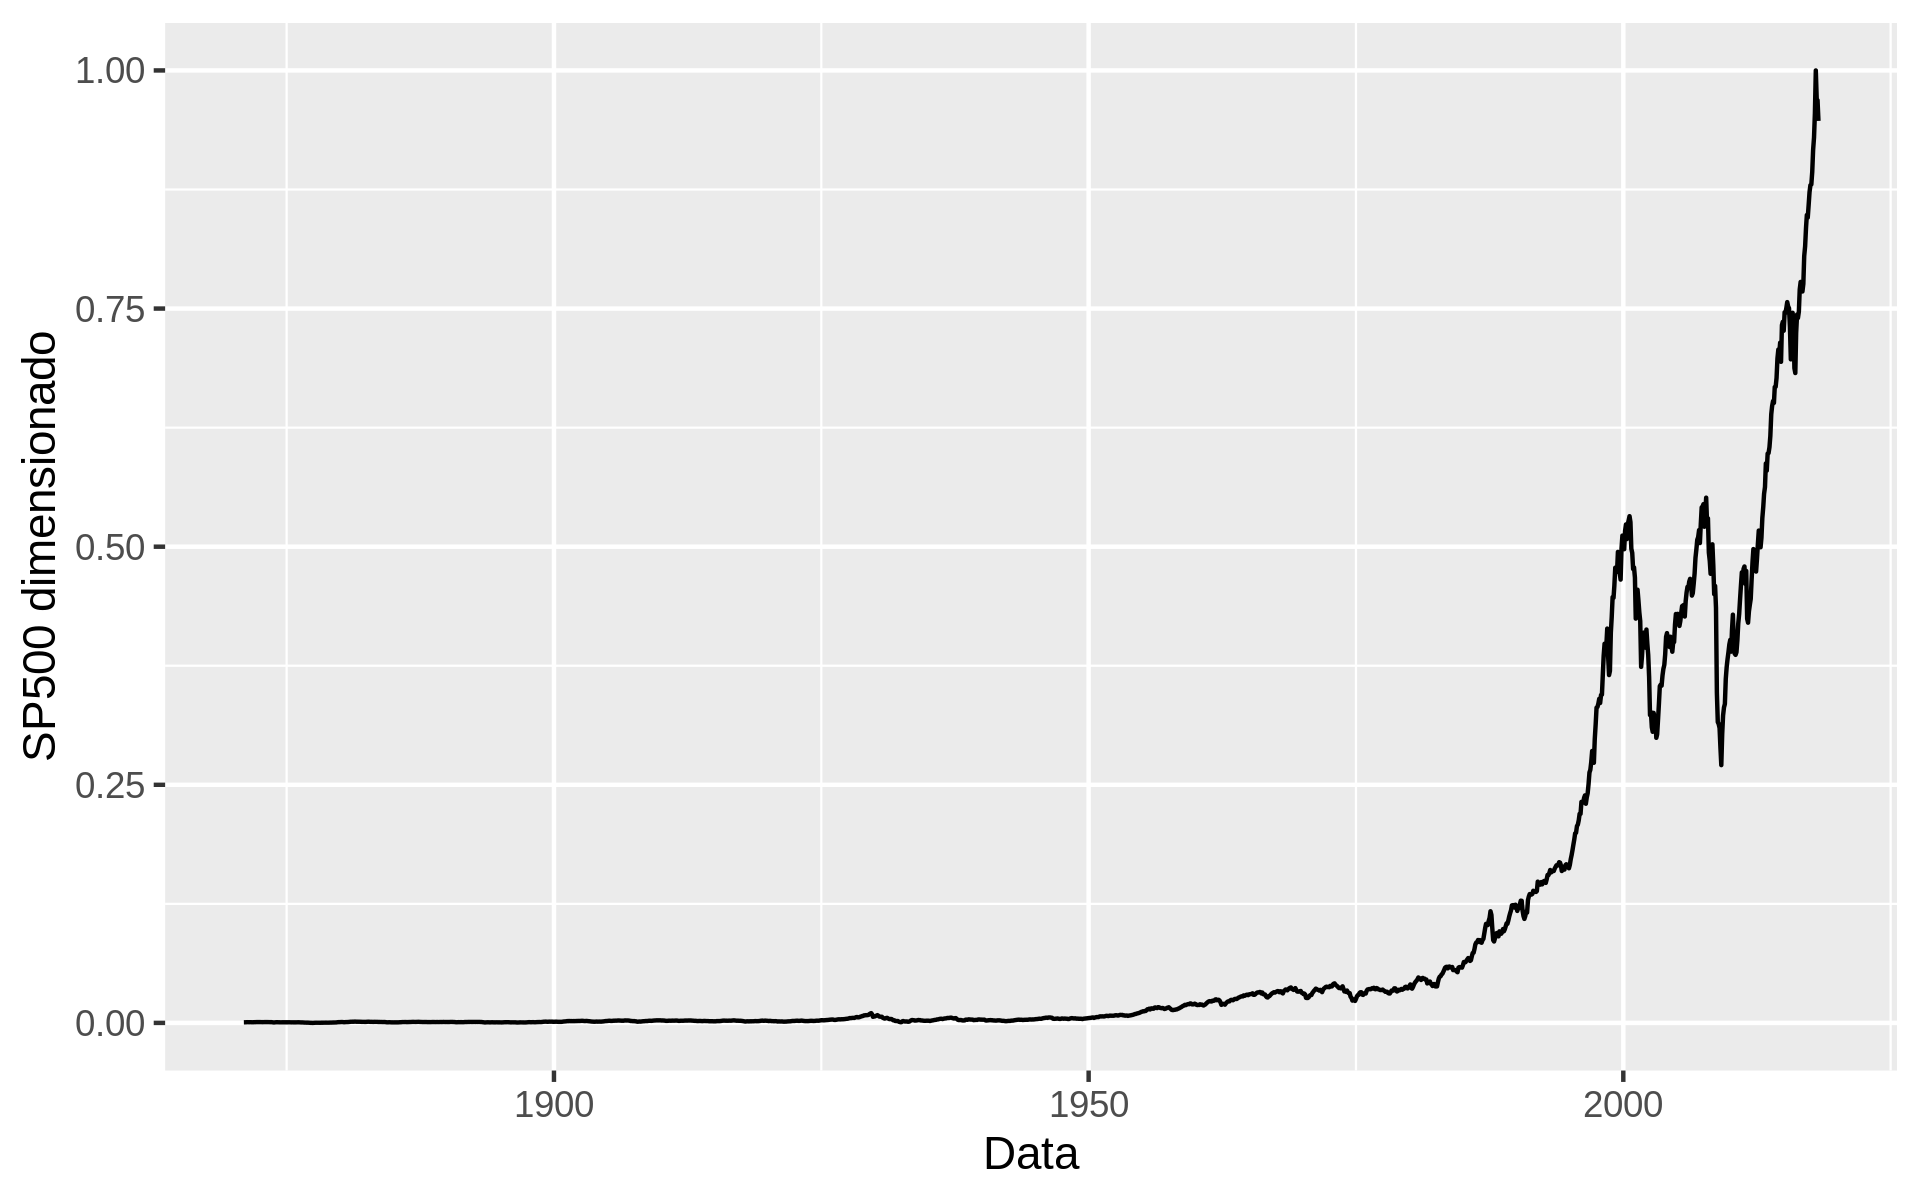
\includegraphics[width=.5\linewidth]{images/SP500.png}
    \source{Elaborado pelo autor}
\end{figure}

A  divisão do  conjunto  de treino  e  teste  foi realizado  de  maneira a  ser
utilizado 70\% dos  dados durante o treinamento e 30\%  durante a validação. Na
\autoref{fig:traintest} estes conjuntos são descritos.

\begin{figure}[ht]
    \caption{Divisão da série entre os conjuntos de treino e teste}\label{fig:traintest}
    \begin{subfigure}{.5\textwidth}
        \centering
        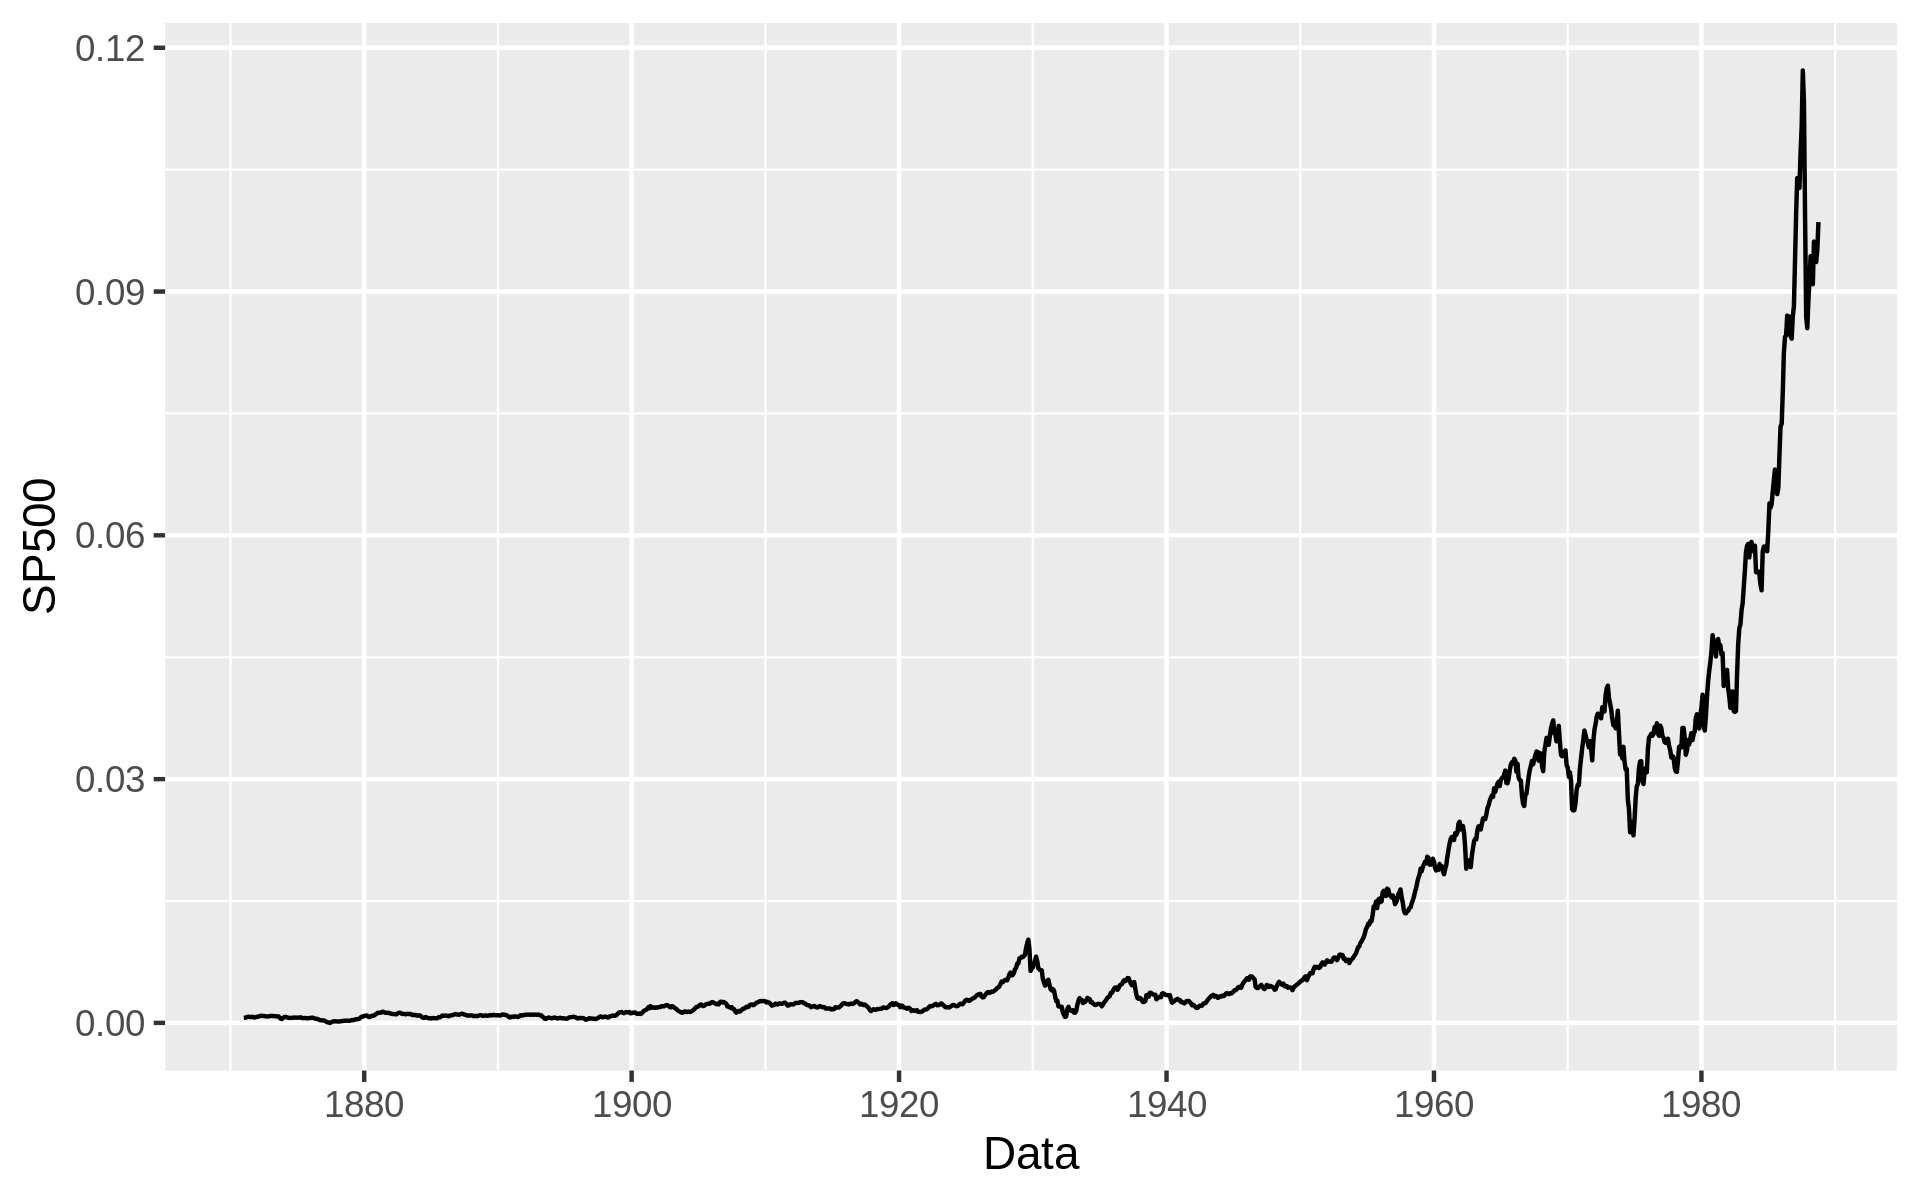
\includegraphics[width=.8\linewidth]{images/SP500_train.png}
        \caption{Conjunto de treino}
    \end{subfigure}
    \begin{subfigure}{.5\textwidth}
        \centering
        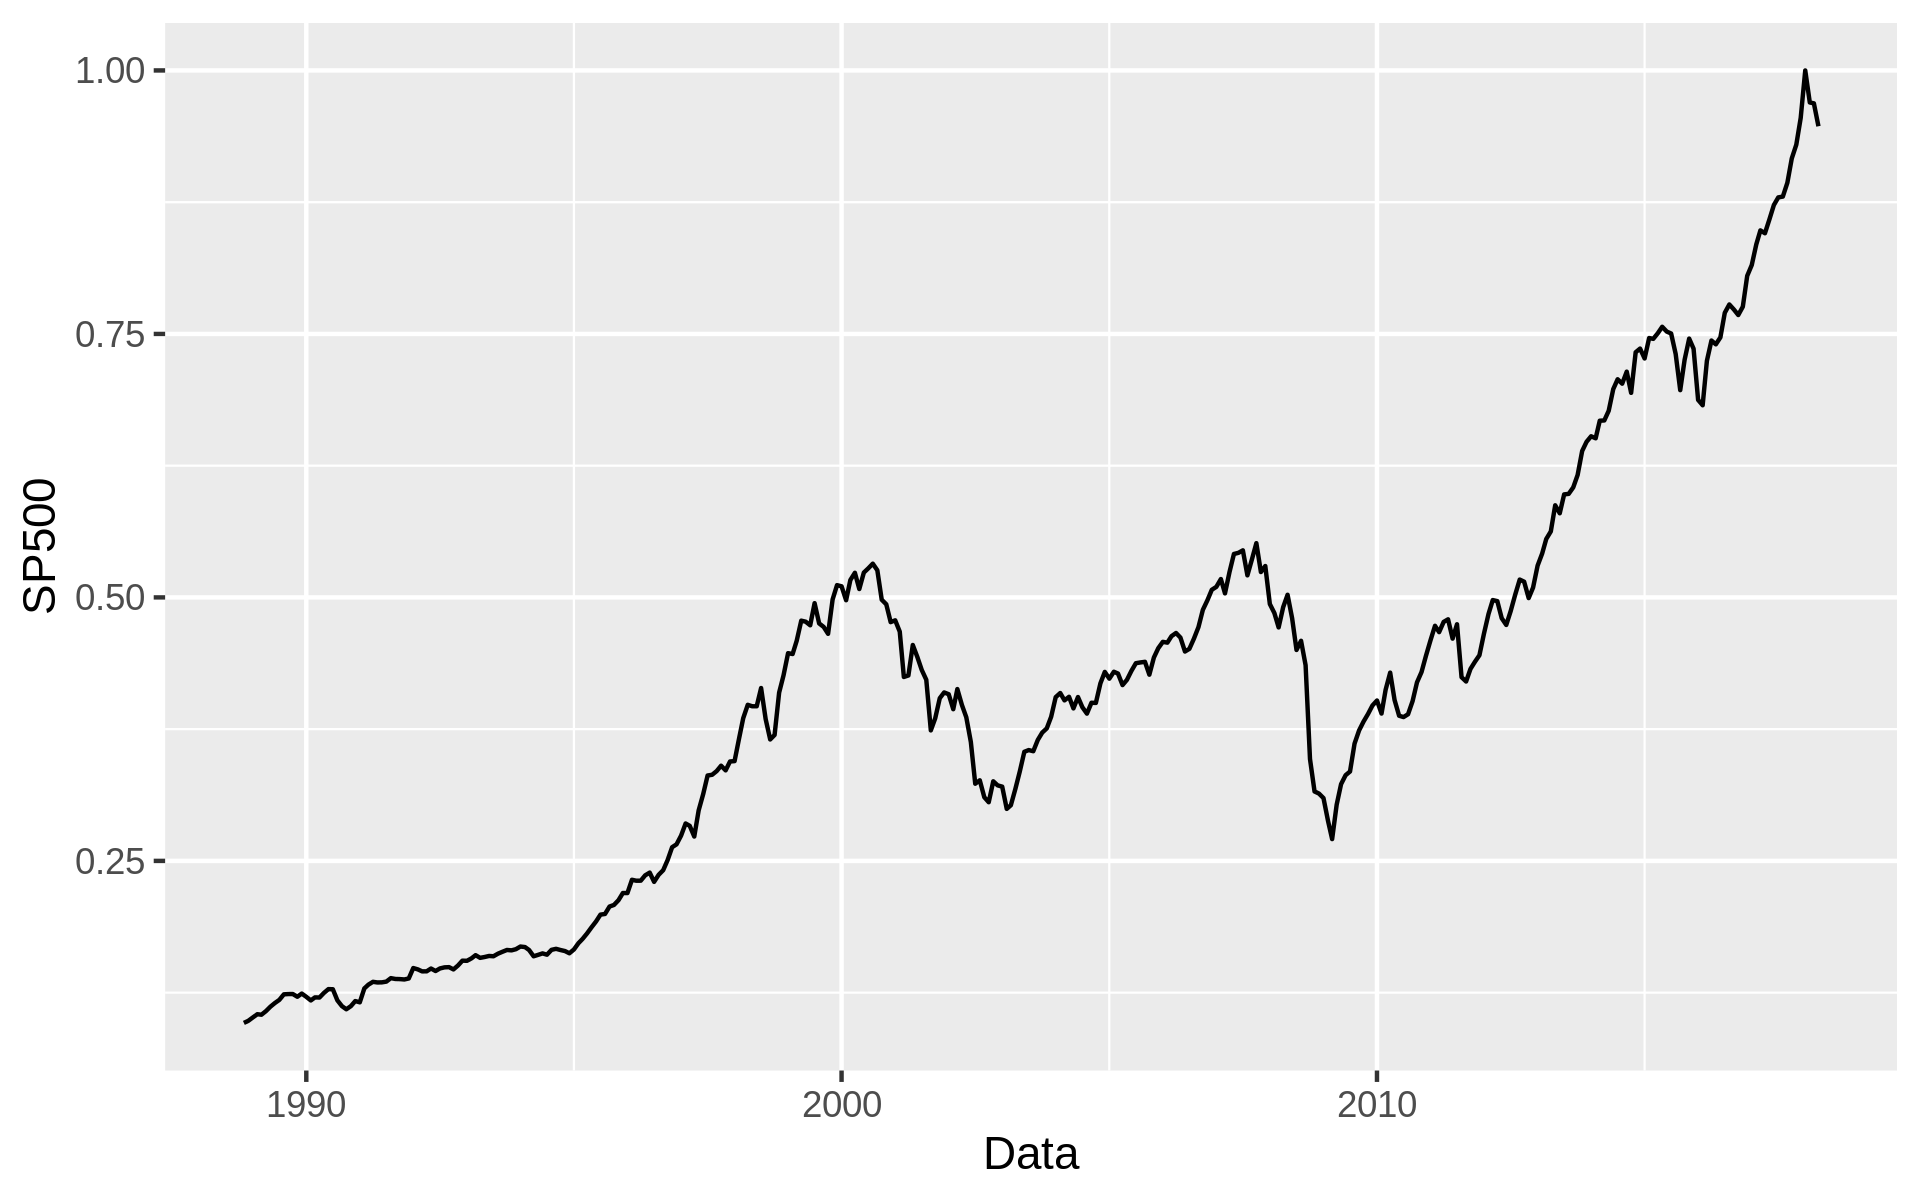
\includegraphics[width=.8\linewidth]{images/SP500_test.png}
        \caption{Conjunto de teste}
    \end{subfigure}
    \source{Elaborado pelo autor}
\end{figure}

Após a análise, foram encontrados os modelos  que mais se adequam à série e foi
validada  a capacidade  deste  modelo  prever um  dia  adiante.  Para tornar  a
comparação justa,  foi definido que  a quantidade de observações  utilizadas na
camada  de entrada  do modelo  de  redes neurais  fosse semelhante  a ordem  do
processo autorregressivo.

\section{Análise da série}

Seguindo  as etapas  para construção  do modelo,  foi realizada  a análise  dos
dados.  O  objetivo  era  identificar  as  características  da  série,  como  a
estacionariedade, e  quanto a  existência de  tendência e  sazonalidade. Sendo,
também, já  realizada a remoção  de \textit{outliers} que possam  atrapalhar na
construção do modelo.

Já na  análise dos gráficos da  série, na \autoref{fig:sp500}, fica  evidente a
existência de  tendência, permitindo concluir  que a série não  é estacionária.
Conclui-se  isso, também,  a partir  da análise  da \autoref{fig:acfsp500}  que
demonstra a  existência de um  grande número  de correlações positivas  fora do
intervalo de confiança.

\begin{figure}[ht]
    \centering
    \caption{Função de autocorrelação para a série S\&P500}\label{fig:acfsp500}
    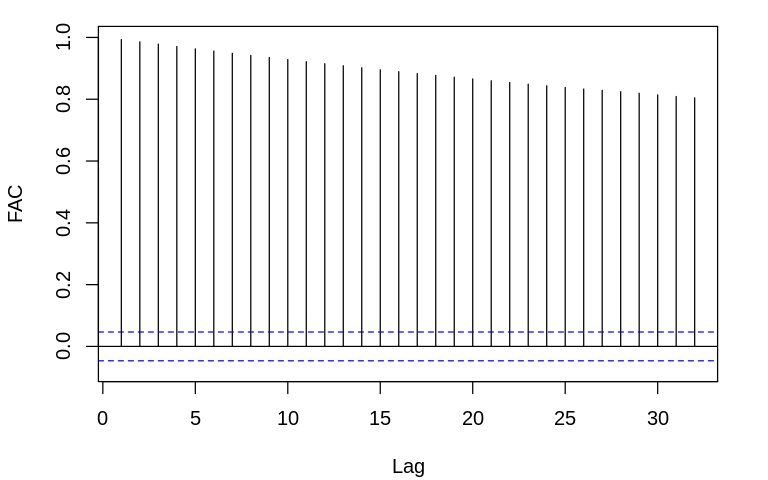
\includegraphics[width=.5\linewidth]{images/SP500_FAC.png}
    \source{Elaborado pelo autor}
\end{figure}

Para  tornar  a série  estacionária,  é  necessário realizar  inicialmente  uma
diferenciação.  Tem-se, na  \autoref{fig:sp500diff}, a  primeira diferenciação.
Pela  observação  da  função autocorrelação,  na  \autoref{fig:acf_diff_sp500},
pode-se concluir que uma única diferenciação foi suficiente.

\begin{figure}[ht]
    \centering
    \caption{Primeira diferenciação dos dados do S\&P500}\label{fig:sp500diff}
    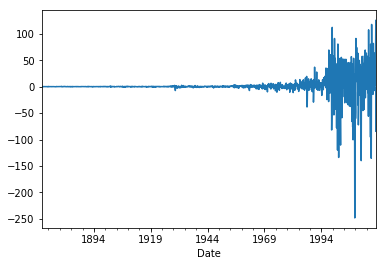
\includegraphics[width=.5\linewidth]{images/sp500diff.png}
    \source{Elaborado pelo autor}
\end{figure}

\begin{figure}[ht]
    \centering
    \caption{Função de autocorrelação da série S\&P500 diferenciada uma vez}\label{fig:acf_diff_sp500}
    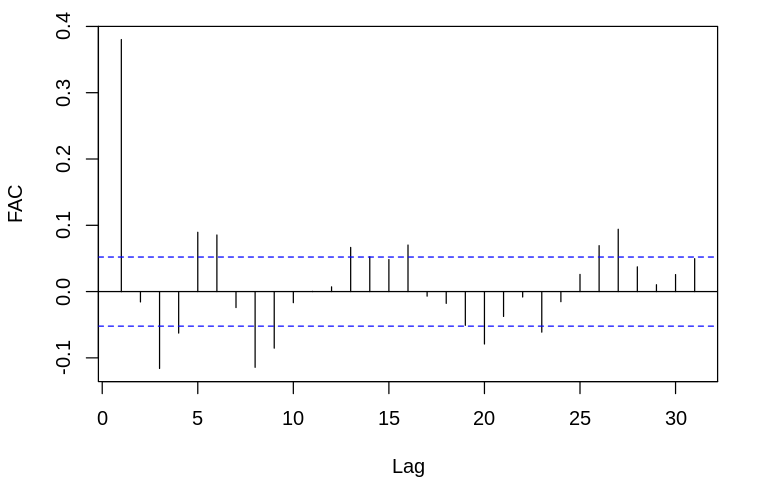
\includegraphics[width=.5\linewidth]{images/SP500_diff_FAC.png}
    \source{Elaborado pelo autor}
\end{figure}

Quanto à sazonalidade, pode-se observar a  existência de um padrão que remete a
um comportamento na  \autoref{fig:acf_diff_sp500}. No entanto, não  é tão claro
qual o período. Para se definir  isso, seria necessária a definição de técnicas
que não fizeram parte desse trabalho.

Realizada a  análise, pode-se  concluir que  o modelo  ARMA sem  integração não
seria  suficiente.  Assim, o  parâmetro  $d$  do  modelo  ARIMA será  de  ordem
1,  devido  a  ter  sido  necessária uma  diferenciação  para  tornar  a  série
estacionária.

\section{Definição do modelo probabilístico}

Compreendido  o  comportamento  da  série, definiu-se  a  correlação  entre  as
observações  para  possibilitar a  construção  do  modelo probabilístico.  Isso
foi  feito   usando  do  gráfico   da  função  de   autocorrelação  apresentado
na  \autoref{fig:acf_diff_sp500}  em  conjunto  com  o  gráfico  da  função  de
autocorrelação  parcial   da  \autoref{fig:sp500pacf}.  Segundo  o   modelo  de
\citeonline{box}, deve-se analisar o modelo com $p$ sendo 1, 2 ou 5, e para $q$
sendo 1, 2 ou  7. A seleção do melhor modelo foi dado  utilizando o critério de
informação de Akaike.

\begin{figure}[ht]
    \centering
    \caption{Função de autocorrelação parcial da série diferenciada S\&P500}\label{fig:sp500pacf}
    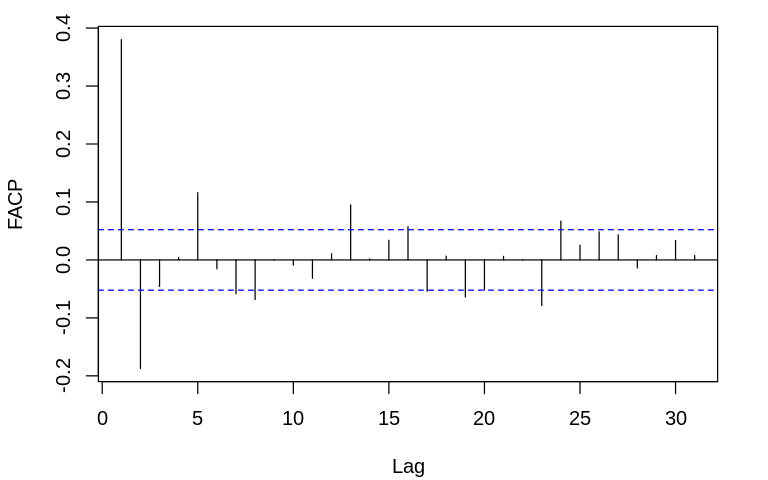
\includegraphics[width=.5\linewidth]{images/SP500_diff_FACP.png}
    \source{Elaborado pelo autor}
\end{figure}

A \autoref{tab:aicarima} apresenta as métricas AIC para os modelos propostos e,
em  destaque, o  modelo com  melhor  resultado. Logo,  o modelo  probabilístico
utilizado para comparar o desempenho foi o ARIMA(5,1,7).

\begin{table}[ht]
\centering
    \caption{Tabela de modelos testados para $p$ e $q$ no modelo ARIMA($p$, 1, $q$)}\label{tab:aicarima}
\begin{tabular}{l c c c}
                        & \multicolumn{3}{c}{$q$}           \\
    $p$                 & 1      & 2      & 7               \\
    \toprule
    1                   & -15953 & -15952 & -15979          \\
    2                   & -15965 & -15968 & -15989          \\
    5                   & -15984 & -15988 & \cellcolor[HTML]{AAAAAA}\textbf{-16004} \\
\end{tabular}
\source{Elaborado pelo autor}
\end{table}

Para ser  possível concluir o modelo  como bom, deve-se, ainda,  analisar se as
funções de autocorrelação e de autocorrelação parcial dos resíduos apresentam a
existência  de  correlações significativas.  Na  \autoref{fig:acffigresiduals},
vemos que  existem ainda correlações  relevantes. No entanto, são  geradas pela
componente sazonal  da série  e, como  já dito, não  fizeram parte  do objetivo
deste trabalho.

\begin{figure}[ht]
    \caption{Funções de autocorrelação e de autocorrelação parcial dos resíduos do
    modelo ARIMA(5,1,7) para a série S\&P500}\label{fig:acffigresiduals}
    \begin{subfigure}{.5\textwidth}
        \centering
        \caption{Função de autocorrelação dos resíduos}
        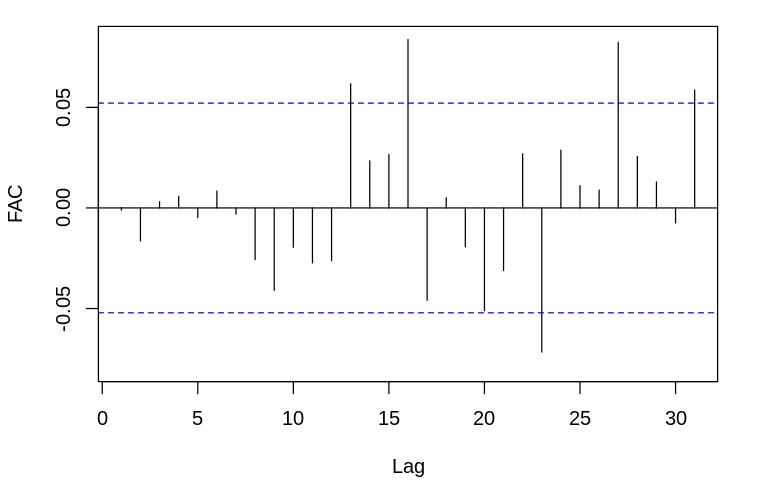
\includegraphics[width=.8\linewidth]{images/residuals_FAC.png}
    \end{subfigure}
    \begin{subfigure}{.5\textwidth}
        \centering
        \caption{Função de autocorrelação parcial dos resíduos}
        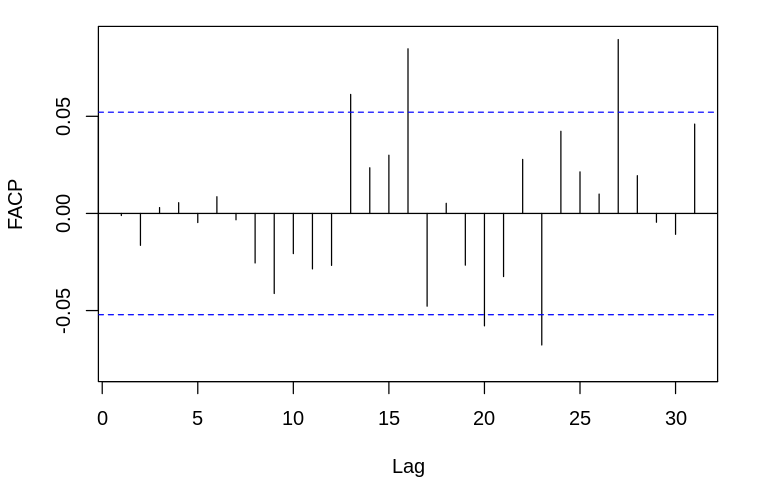
\includegraphics[width=.8\linewidth]{images/residuals_FACP.png}
    \end{subfigure}
    \source{Elaborado pelo autor}
\end{figure}

\section{Definição do modelo utilizando aprendizado de máquina}

Já para o  desenvolvimento do modelo neural, não foi  necessária uma observação
profunda da  série. No entanto,  exigiu uma parametrização muito  mais complexa
do  modelo.  Observado como  o  modelo  convergia, considerando  os  parâmetros
escolhidos, foi realizada uma busca em grade extensiva para encontrar um modelo
com melhor capacidade representativa.

Na \autoref{tab:gridsearch},  observamos todos os parâmetros  testados na busca
em grade.

\begin{table}[ht]
\centering
\caption{Parâmetros utilizados na busca em grade}\label{tab:gridsearch}
\begin{tabular}{l l}
\multicolumn{1}{c}{Parâmetro}        & \multicolumn{1}{c}{Possibilidades}  \\
    \toprule
    Número de camadas                & 1 \ldots 4                          \\
    Número de unidades por camada    & 1 \ldots 20                         \\
    $\lambda$ regularização          & 0.00001 \ldots 0.0001               \\
    Função de ativação               & $relu$, $sigmoid$                   \\
    Função de perda                  & MSE, MAE                            \\
    Iterações                        & 20 \ldots 500
\end{tabular}
\source{Elaborado pelo autor}
\end{table}

Uma característica  que foi logo  observada nas primeiras  execuções anteriores
da  aplicação da  regularização  foi  o rápido  \textit{overfit}  nos dados  de
treinamento, como  visto na  \autoref{fig:sp500_overfit}. Apesar de  aplicado a
validação  cruzada. Logo,  a  aplicação da  regularização  foi suficiente  para
diminuir a ocorrência do \textit{overfit}.

\begin{figure}[ht]
    \centering
    \caption{Gráfico da comparação dos valores previsto e reais para o conjunto de treino e teste}\label{fig:sp500_overfit}
    \minipage{0.50\linewidth}
        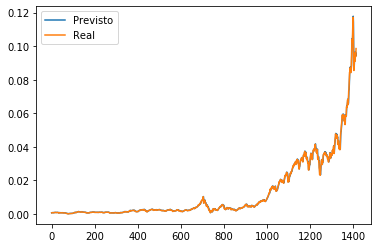
\includegraphics[width=\linewidth]{images/sp500_overfit_train.png}
    \endminipage\hfill
    \minipage{0.50\linewidth}
        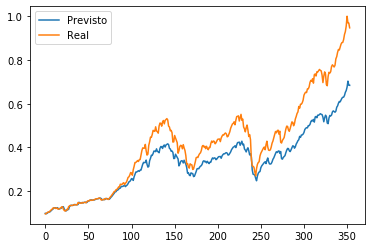
\includegraphics[width=\linewidth]{images/sp500_overfit_test.png}
    \endminipage\hfill
    \source{Elaborado pelo autor}
\end{figure}

\begin{figure}[ht]
    \centering
    \caption{Gráfico da função de perda em  função do números de iterações para
    a série S\&P500}\label{fig:iter_sp500_overfit}
    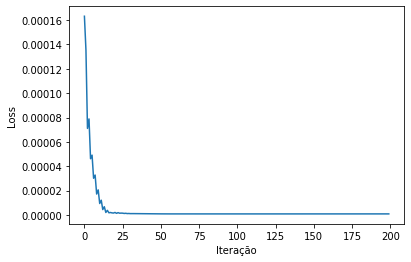
\includegraphics[width=.5\linewidth]{images/sp500_overfit_iter.png}
    \source{Elaborado pelo autor}
\end{figure}

O modelo  de redes neurais artificiais  selecionado a partir da  busca em grade
foi  com duas  camadas. A  primeira camada  com 13  neurônios e  a segunda  com
somente um neurônio, já que esta é a  camada de saída. A função de ativação foi
a $relu$  e o  $\lambda$ da  regularização ficou como  $0.000001$. A  função de
perda selecionada foi a função média  dos erros quadrados e 300 iterações foram
suficientes. Já que  o modelo probabilístico tem  $p$ igual a 5,  foi fixado em
cinco observações a realização da previsão.

\chapter{Resultados}\label{chap:result}

A  partir dos  modelos gerados,  foram  obtidos os  resultados apresentados  na
\autoref{tab:resultadosp500},  e o  gráfico  do conjunto  de testes  comparando
os   resultados  obtidos   com  os   valores  previstos   estão  dispostos   na
\autoref{fig:comparesp500}.  Considerando  que  as linhas  se  sobrepuseram  em
praticamente todo o gráfico, foi gerado  também o gráfico dos erros de previsão
acumulados, na  \autoref{fig:cumsumsp500}. Utilizando  o gráfico de  erros fica
mais claro  como os dois modelos  progridem na previsão da  série, demonstrando
que as duas se mantiveram coerentes durante todo o conjunto, sem demonstrar uma
perda desempenho em momentos de maior variação das observações.

A partir dos os resultados, fica claro que os dois modelos conseguiram êxito na
tarefa de aproximar o comportamento da  série. Em termos comparativos, o modelo
neural obteve resultado um pouco inferior, na ordem de $0,6\%$.

\begin{table}[ht]
    \centering
    \caption{Valores do erro para a série S\&P500}\label{tab:resultadosp500}
    \begin{tabular}{ll}
        \multicolumn{1}{c}{Modelo} & \multicolumn{1}{c}{MSE} \\
        \toprule
        MLP                        & 0,0002101               \\
        ARIMA                      & 0,0002088
    \end{tabular}
    \source{Elaborado pelo autor}
\end{table}

\begin{figure}[ht]
    \caption{Comparativos dos resultados}\label{fig:comparesp500}
    \begin{subfigure}{.5\textwidth}
        \caption{Gráfico comparativo entre os modelos obtidos}\label{fig:comprealsp500}
        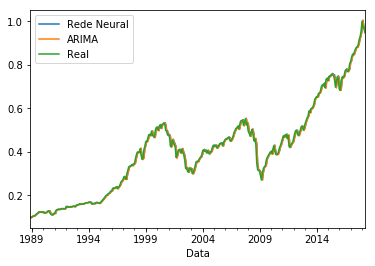
\includegraphics[width=.8\linewidth]{images/sp500_prediction_compare.png}
    \end{subfigure}
    \begin{subfigure}{.5\textwidth}
        \caption{Gráfico dos erros acumulados}\label{fig:cumsumsp500}
        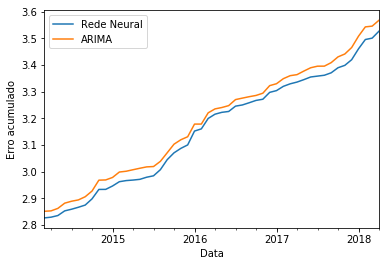
\includegraphics[width=.8\linewidth]{images/sp500_cumsum.png}
    \end{subfigure}
    \source{Elaborado pelo autor}
\end{figure}

Uma possível  explicação para  a semelhança dos  resultados pode  ser explicada
pela aparente semelhante entre um  \textit{perceptron}, utilizado em uma tarefa
de aprendizado,  e um regressor que  é base tanto do  processo autoregressivo e
do  de  médias  móveis.  Mais  claramente  ainda  se  observarmos  um  processo
autoregressivo  de  ordem 1,  dado  matematicamente  $X_t =  \alpha_1X_{t-1}  +
\epsilon_t$, é bastante semlhante a  um \textit{perceptron}, $X_t = o(X_{t-1} *
w_1 + w_0)$,  permitindo até mesmo traçar equivalências, como  os pesos da rede
neural, $w$, serem equivalentes aos coeficientes $\alpha$.

Outra  forma  que  podemos  compreender  os modelos  é  a  simplicidade  de  se
obtê-los. Para o ARIMA, foi necessária diversas observações do comportamento da
série,  e embora  não tenha  sido  o caso,  este  modelo é  muito suscetível  a
observações falhas, \textit{outliers}, que  podem demandar etapas anteriores de
pré processamento. Enquanto  que modelos utilizando redes  neurais não demandam
do usuário um grande conhecimento do comportamento ou pré processamento, já que
sua natureza  não linear é  capaz de aprender  por reconhecimento de  padrões o
comportamento  da série.  Uma  característica  inerente aos  dois  modelos é  a
complexidade do ajuste dos parâmetros, enquanto para o modelo probabilístico se
dá por da analise da serie, no modelo neural ocorre seguindo o comportamento da
etapa de aprendizado.

\chapter{Conclusões}\label{chap:concl}

O objetivo deste trabalho foi produzir e avaliar modelos preditivos para séries
temporais utilizando  algoritimos estatísticos e  de aprendizado de  máquina. É
comum  em  trabalhos, a  utilização  de  métodos  probabilísticos quando  se  é
realizada  a tarefa  de  previsão  de séries.  Mais  especificamente, o  modelo
hibrido ARIMA  proposto por \citeonline{box}.  No entanto, modelos  baseados em
algoritimos de  aprendizado de máquina  se tornaram notórios nos  últimos anos.
Logo,  neste trabalho,  foram comparados  estes modelos  para entender  as suas
capacidades e observar os seus desafios particulares.

Para  permitir a  avaliação, foi  necessária  a compreensão  da construção  dos
modelos.  O proposto  por  \citeonline{box} apresentou  uma complexidade  muito
superior na etapa  de análise da série,  já que esse modelo  pode ser entendido
como  dependente  de  diversas  intervenções  para  melhor  parametrização.  Já
o  modelo  de  aprendizado,  utilizando redes  neurais  de  múltiplas  camadas,
apresentou  uma  necessidade mínima  de  compreensão  dos dados  estudados.  No
entanto, sua complexidade se apresentou durante a etapa de treinamento.

Quanto aos resultados,  pôde-se concluir que os modelos  utilizados foram muito
similares  em  seus  desempenhos.  Vale  notar  que  os  resultados  não  foram
expressivos  na conclusão  de  superioridade  de um  modelo.  Quanto à  métrica
utilizada para a avaliação, o modelo ARIMA teve resultado superior em uma ordem
ínfima, 0,6\%, em relação ao modelo de redes neurais.

Os modelos probabilísticos  obtidos foram um modelo hibrido ARMA  de ordem 5 do
processo autorregressivo e de ordem 7  para o processo de médias móveis. Também
foi  necessária uma  diferenciação, já  que a  série apresentou  tendência. Por
conta disso,  foi necessária a  diferenciação para  para obtenção de  uma série
estacionária, característica requerida pelo modelo ARMA\@.

Para obtenção do  modelo de redes neurais,  a mudança dos dados  se resumiram a
realizar de um dimensionamento para um intervalo de valores. Sem ser necessário
maior  avaliação   do  comportamento,  já  que,   segundo  \citeonline{haykin},
algoritimos de aprendizado são ditos dirigido  por dados. No entanto, durante a
etapa  de treinamento  foi  necessária  a realização  de  diversos testes  para
encontrar  o modelo  que melhor  se adequava,  além da  aplicação de  validação
cruzada e  regularização para  diminuir a  ocorrência de  \textit{overfit}. Por
meio  desse processo,  identificou-se uma  rede neural  de duas  camadas: a  de
entrada com  13 unidades de  processamento, \textit{perceptron}, e a  segunda a
camada de  saída com  um único  neurônio, representando a  previsão um  passo a
diante.

Conclui-se, então,  que os modelos são  suficientes para a tarefa.  No entanto,
deve-se observar que os modelos  estatísticos tornam a parametrização uma etapa
muito mais  complexa que o  modelo de aprendizado.  Assim, a escolha  do modelo
pode ser feita analisando capacidade de análise de quem o constrói, ou conforme
o comportamento dos dados no caso do uso de redes neurais artificiais.

\section{Trabalhos futuros}

Um  possível trabalho  futuro é  a  avaliação de  diferentes modelos  híbridos.
Aproveitando-se  da  capacidade  dos  modelos  probabilísticos  em  representar
comportamento  linear  e,  também,  a  capacidade  de  modelos  de  aprendizado
em  séries não  lineares, como  feito por  \citeonline{oCaraLaDoModeloHibrido}.
Uma  outra possibilidade  é  a  utilização de  redes  neurais recorrentes,  que
se  diferenciam  de  modelos  \textit{feedforward}  por  possuir  memorio.  Uma
arquitetura de  redes neurais  que tem  apresentado bons  resultados é  a LSTM.
Alguns  trabalhos, como  \citeonline{oDoCaraQueComparaArimaComLSTM}, demonstram
que  é  possível  obter  resultados   superiores  com  sua  aplicação.  Podemos
ainda  estudar essas  comparações  com séries  de  comportamento diferente,  e,
consequentemente, utilizar  modelos estatísticos mais completos,  como o SARIMA
ou SARIMAX\@.

\postextual

\bibliography{referencias}

\end{document}
